% =====================================================================================
% Paper 3 — FULL-LENGTH (expanded). Fork; data-driven design-tool paper; distinct from paper 2.
% Conventions: Times (newtxtext/newtxmath); typeset math; NO total-loss plot; reproducibility table;
% REAL citations only (all verified); honest scope. Self-contained.
% =====================================================================================
\documentclass[11pt]{article}
\usepackage[T1]{fontenc}
\usepackage{newtxtext,newtxmath}
\usepackage{amsmath,mathtools,bm}
\usepackage{siunitx}
\usepackage{graphicx}
\usepackage{float}
\usepackage{booktabs}
\usepackage{algorithm}
\usepackage{algpseudocode}
\floatstyle{ruled}\restylefloat{algorithm}  % ruled header bar + top/bottom rules (table-like)
\usepackage[margin=1in]{geometry}
\usepackage[hidelinks]{hyperref}
\newcommand{\im}{\mathrm{j}}
% Float placement: let large floats share pages with text and require float pages to be
% nearly full, so no half-empty float page is created (reduces page whitespace).
\renewcommand{\topfraction}{0.92}
\renewcommand{\bottomfraction}{0.85}
\renewcommand{\textfraction}{0.06}
\renewcommand{\floatpagefraction}{0.85}
\setcounter{topnumber}{3}
\setcounter{bottomnumber}{2}
\setcounter{totalnumber}{5}
% =====================================================================================
% PROPOSED HIGHLIGHTS for EAAI submission (separate Highlights file; 3-5 bullets, <=85 chars
% incl. spaces). Do NOT place in the manuscript body; authors copy these into the system.
% (Each line below verified <=85 characters; ordered novelty-first for the editor.)
%   - Resonance-aware active sampling beats every off-the-shelf acquisition rule
%   - Learns a 24-GHz reflectarray cell surrogate from ~16 full-wave anchors, no oracle
%   - The advantage transfers across 3 cell types and to non-electromagnetic resonances
%   - Differentiable surrogate gives full-wave gradients; inverse design to 0.9 deg
%   - A total-field Maxwell-residual (PINN) term is unnecessary and counterproductive
% =====================================================================================
\title{\bfseries Resonance-Aware Active Sampling for Data-Efficient Differentiable Surrogates
of Resonant Responses: A Reflectarray Unit-Cell Case Study}
\author{Long Zhang\,$^{*}$,\quad Xuan Shi,\quad Liang Ma,\quad Shengjun Wu,\quad Kai You,\quad Zijuan Wu\\[2pt]
\small Hubei University of Automotive Technology, Shiyan 442002, China\\
\small $^{*}$Corresponding author: Long Zhang (20230100@huat.edu.cn); ORCID \texttt{0009-0004-4109-6587}}
\date{}
\begin{document}
\maketitle

\begin{abstract}
\noindent
Many design problems in radio-frequency, photonics, and metamaterial engineering reduce to learning an
expensive-to-sample, \emph{resonance-dominated} response, in which a sharp, high-$Q$ feature rotates the
output over a narrow design window---costly to simulate and hard for physics-informed neural networks
(PINNs). We develop a resonance-aware active-learning methodology: a curvature-driven acquisition that
concentrates a scarce full-wave budget on the resonance, coupled to a \emph{differentiable surrogate} that
yields design gradients. On 24-GHz reflectarray unit cells, a \emph{deployable} online acquisition---scoring
candidates using only already-acquired anchors, no oracle---learns the two-parameter reflection-phase
surface to sub-degree resonance error from $\mathcal{O}(10)$ full-wave anchors and beats both textbook
Gaussian-process uncertainty sampling and a published adaptive sampler (LOLA--Voronoi); an idealised oracle
that scores on the full surface bounds the achievable placement from above (a steeper $N^{-2.1}$ decay
versus uniform sampling's $N^{-0.8}$). The advantage recurs across three reflectarray topologies and,
changing only the oracle, transfers to two non-electromagnetic resonances---evidence it is a reusable method
for resonance-dominated responses, not a one-off heuristic. The surrogate's
gradients agree with full wave and drive inverse design to a \SI{0.9}{\degree} average error. A controlled
ablation shows a \emph{total-field} Maxwell-residual term is unnecessary and counterproductive here---the
lever is data placement, not the physics residual. The artificial-intelligence contribution is this
resonance-aware sampling-plus-differentiable-surrogate methodology; the engineering application is low-cost,
gradient-based characterisation and inverse design of resonant reflectarray/metasurface unit cells. All
claims are scoped to this simulated cell class.
\end{abstract}

\noindent\textbf{Keywords:} active learning; differentiable surrogate; physics-informed neural network;
inverse design; reflectarray; metasurface unit cell.

\section{Introduction}
A recurring problem for machine learning in the physical sciences is to build a fast, accurate, and
ideally \emph{differentiable} surrogate of an \emph{expensive-to-sample, resonance-dominated} parametric
response---one whose output rotates through its full range over a narrow window of the design variables
because of a sharp, high-$Q$ resonance. Such responses arise across photonics, RF, and metamaterials, and
they stress two of the most active lines in scientific machine learning: \emph{active learning}, which must
decide where to spend a scarce simulation budget, and \emph{physics-informed} losses, whose benefit is
uncertain precisely for stiff, high-frequency solutions. This paper studies that AI problem and uses a
reflectarray unit cell as a concrete, fully validated testbed.
Coded metasurfaces and reflectarrays synthesise a target aperture field by assigning each sub-wavelength
cell a prescribed reflection phase through its
geometry~\cite{trentini1956,cui2014,reflectarray2022,li2021codingreflector}. The same per-cell
phase-synthesis task underlies transmitarrays and Huygens
metasurfaces~\cite{abdelrahman2015transmitarray,epstein2014huygens}: in every case the designer must
know, accurately and at low cost, how a cell's complex reflection (or transmission) coefficient depends
on its dimensions, and increasingly must \emph{differentiate} that dependence so that gradient-based
inverse design~\cite{liu2018,molesky2018} can place hundreds of cells at once. (Adjoint sensitivities give
exact full-wave gradients~\cite{molesky2018} but require a bespoke solver-coupled implementation per
problem; a differentiable surrogate instead yields reusable geometry gradients from a few black-box solver
calls, which is what we pursue here.) The bottleneck is that the cell response is governed
by a sub-wavelength resonance: as the resonant dimension is swept, the reflection phase rotates rapidly
through the full design range over a narrow geometric window, and it is exactly this sharp, high-$Q$
feature that makes the response both expensive to characterise and awkward to model.

The standard route is to build a look-up library by full-wave sweeping, which is accurate but scales
poorly with the number of geometric parameters. Data-driven surrogates remove the per-query solve---both
neural-operator models that learn the solution map~\cite{ludeeponet2021,li2021fno,augenstein2023} and
supervised networks for photonic and antenna response~\cite{jiang2021,koziel2024surrogate}---but their
training cost grows with dimensionality~\cite{sarker2023mlreview}, which \emph{active-learning} surrogates mitigate by
sampling where the model is least certain~\cite{settles2012,lookman2019}---a strategy shown to cut the
number of simulations by more than an order of magnitude for photonic-surface
surrogates~\cite{pestourie2020}. Yet generic
uncertainty-driven acquisition is not tailored to the structure that makes these responses hard: a
\emph{localised} resonance that dominates both the cost and the design-relevant phase, and that couples
awkwardly to the second AI ingredient a designer needs---a surrogate whose geometry gradients are
trustworthy enough to drive inverse design. A second route is the
data-free physics-informed neural network (PINN), which minimises the Maxwell residual and
needs no training data at all~\cite{raissi2019,karniadakis2021}, including parametric and electromagnetic
variants~\cite{beltran2022,nohra2024pinnem}. PINNs are,
however, known to struggle with sharp, high-frequency, or stiff
solutions~\cite{krishnapriyan2021,wang2021ntk,wanggrad2021}, and the sub-wavelength cell resonance is
precisely such a feature; whether a physics-informed loss helps or hurts a \emph{sparse-data} surrogate in
this regime is, to our knowledge, untested at the device level. The methodological gap we address is
therefore at the intersection of these AI lines---resonance-aware active learning, differentiable
surrogates that yield physically consistent gradients, and a quantified account of when a physics-informed
loss helps or hurts---and it crystallises in one concrete, answerable question on the testbed: \emph{for
the resonant reflection response, does adding the Maxwell residual help a sparse-data surrogate, or is
well-placed data enough on its own?}

\emph{The novel claim of this paper, in one sentence, is the following.} Where generic adaptive sampling
chooses points by response curvature/error, Gaussian-process posterior variance, or LOLA--Voronoi
space-filling~\cite{settles2012,crombecq2011,gramacy2020}, we identify the \emph{resonance class} of
expensive responses and give an acquisition tailored to it---one that deliberately \emph{crowds} the narrow
high-$Q$ band that those space-filling rules dilute---and we establish it not as a heuristic but as a
characterised method, through (i) a bootstrapped sample-complexity law with confidence intervals, (ii)
cross-domain transfer across three reflectarray topologies and two non-electromagnetic line shapes by
changing only the oracle, (iii) a sampler--learner coupling finding (the clustered anchors that help a
differentiable surrogate hurt a global-kernel model), (iv) an off-grid solver-in-the-loop closure, and (v)
a device-level negative result that a total-field Maxwell residual is counterproductive here. These are one
coherent methodological package for resonance-dominated responses, not five separate observations.

\paragraph{Contributions.} The contributions are methodological---each is an AI/ML method for
expensive-to-sample, resonance-dominated parametric responses, with the 24-GHz reflectarray cell as the
testbed on which it is validated against full wave. The headline is the first: a
\emph{resonance-class} acquisition criterion that beats every off-the-shelf sampler we tested and is shown
to be a reusable, characterised method---not a heuristic---by a bootstrapped sample-complexity law and
cross-domain transfer.
\begin{enumerate}\itemsep1pt
\item A \emph{resonance-aware active-learning acquisition} (a curvature/uncertainty criterion that
concentrates the simulation budget on the localised resonance), together with a \emph{bootstrapped
data-efficiency law} quantifying its sample complexity: paired with a lightweight differentiable
surrogate it captures the full two-parameter response of the testbed cell from $\mathcal{O}(10)$ full-wave
anchors, with a resonance-region error-versus-budget exponent (bootstrap CIs over seeds) steeper than
uniform or random sampling. The method is \emph{deployable}, not oracle-dependent: a fully \emph{online}
variant scoring candidates only on already-acquired anchors retains a steep exponent
($k\!=\!1.73\,[1.49,1.94]$, separated from both uniform and random) and reaches sub-degree resonance
error. The criterion also beats both textbook Gaussian-process uncertainty (maximum-variance) active learning
($\sim\!20\times$) and the standard published adaptive sampler LOLA--Voronoi~\cite{crombecq2011}
($\sim\!7\times$)---both space-fill rather than crowding the resonance---and the advantage \emph{recurs on
two further cell topologies}---a cross dipole (uniform sampling fails entirely) and a harder dual-resonance
cell---and, changing \emph{only the oracle}, \emph{transfers off electromagnetics entirely} to two non-EM
resonance-dominated responses (a driven-oscillator/RLC line shape and a Fano resonance, where uniform again
fails), consistent with the advantage being a property of the acquisition criterion rather than the
patch geometry (Sections~\ref{sec:method}--\ref{sec:eff}, \ref{sec:topology}, \ref{sec:outdomain}).
\item A \emph{differentiable surrogate that yields physically consistent design gradients}: a like-for-like
comparison shows it matches or beats support-vector and plain-network baselines at equal anchor
budgets---its advantage emerging precisely under the clustered active-learning anchors that global-kernel
models handle poorly---and its autodiff geometry gradients agree with full wave and drive a gradient-based
inverse-design loop on the testbed (Sections~\ref{sec:base}--\ref{sec:inv}).
\item A \emph{device-level negative result on physics-informed regularisation}: a controlled ablation
establishes that, for this resonant response, a data-free \emph{total-field} PINN fails and a
physics-informed hybrid is \emph{counterproductive}---a finding that \emph{holds and sharpens} as the
geometry family grows from one to two parameters with scarcer data (hybrid $\sim\!31\times$ worse than
pure data at matched anchors in 2-D)---so well-placed data, not the total-field Maxwell residual, is the
effective lever (Section~\ref{sec:abl}), interpreted through known PINN optimisation
pathologies~\cite{wang2021ntk,wanggrad2021}. The finding is not an artefact of a naive
fixed loss weight: an \emph{advanced} hybrid with NTK/gradient-norm adaptive weighting is still
$\sim\!26\times$ worse than pure data. We do not test a scattered-field reformulation, and we restrict the
claim to total-field formulations.
\end{enumerate}
Three further studies support and delimit these claims. \textbf{(a)~An end-to-end full-wave closure}: cell
sizes from inverting the surrogate's size$\to$phase map realise a phase-gradient metagrating whose full-wave
anomalous reflection is aimed across $\theta\approx11^\circ$--$32^\circ$, tracking generalized Snell's law to
$\approx\!\SI{0.3}{\degree}$---a proof-of-pipeline (angle correct; efficiency $29$--$39\%$, limited by the
single-resonance cell), not a usable-aperture claim (Section~\ref{sec:steer}). \textbf{(b)~A
higher-dimensional study}: on a three-parameter $(L_x,L_y,h)$ cell the data-efficiency advantage widens
(exponent $k\!=\!2.38$ vs $0.50$, non-overlapping 95\% CIs)---but only once the acquisition is
\emph{stratified} along the added axis, a concrete lesson for scaling the method (Section~\ref{sec:3d}).
\textbf{(c)~A transfer result}: pretrained on one substrate, the surrogate warm-starts to a different board
thickness at $\sim\!4\times$ fewer new full-wave anchors than training from scratch
(Section~\ref{sec:transfer}).
The criterion is general in principle---it targets any expensive-to-sample, resonance-dominated
parametric response---and we give first evidence for that generality by transferring it, changing only the
oracle, to two non-electromagnetic line shapes (Section~\ref{sec:outdomain}). The \emph{electromagnetic}
claims, however, remain scoped to the simulated reflection response of three planar reflectarray cell
topologies (a patch, a cross dipole, and a dual-resonance cell) in one full-wave solver, which serves as
the reference throughout; the cost-saving (as opposed to criterion-transfer) results are demonstrated on
that testbed alone.

\begin{figure}[!htbp]\centering
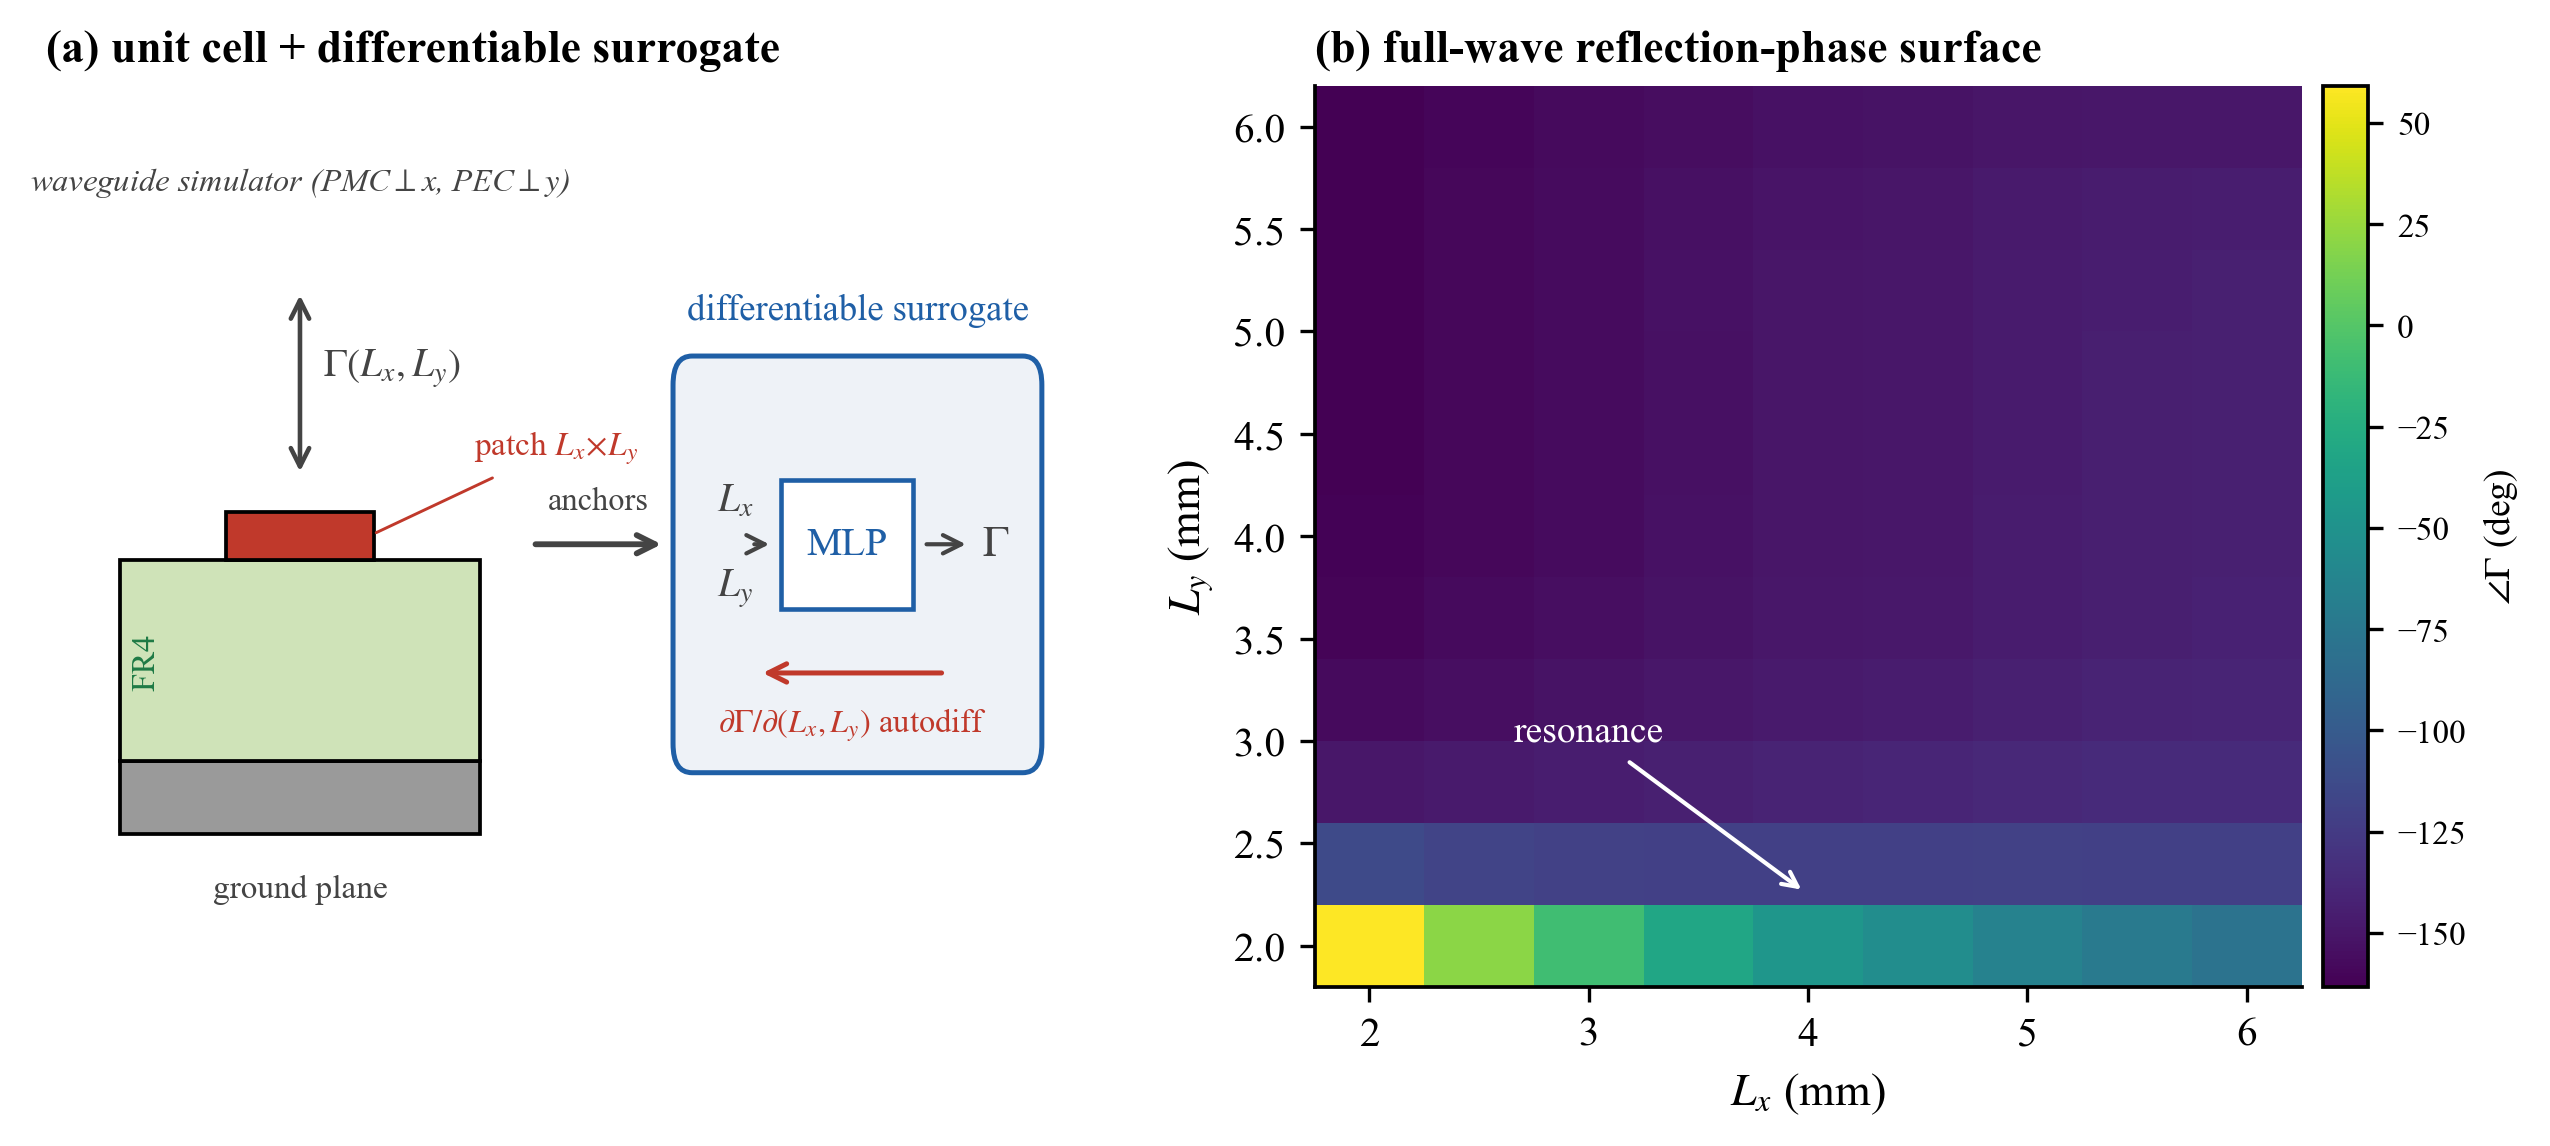
\includegraphics[width=0.97\linewidth]{fig_p3_setup.png}
\caption{(a) Rectangular-patch reflectarray cell in a waveguide simulator and the differentiable
surrogate that maps geometry $(L_x,L_y)$ to the complex reflection $\Gamma$, with autodiff geometry
gradients. (b) The openEMS full-wave reflection-phase surface over $(L_x,L_y)$: a \SI{222}{\degree} swing
whose sharp resonance lies at small resonant length $L_y$ and sharpens as the width $L_x$ narrows.}
\label{fig:setup}
\end{figure}

\section{Problem and full-wave reference}\label{sec:prob}
\paragraph{Unit cell and extraction.} We adopt the standard variable-size patch reflectarray
characterisation~\cite{pozar1997}: a single
rectangular metal patch (transverse width $L_x$, resonant length $L_y$ along the incident
$\mathbf{E}$-field) on grounded FR4 ($\varepsilon_r=4.4$, $\tan\delta=0.02$, thickness \SI{1}{mm}) inside
a \SI{24}{GHz} waveguide simulator with perfect-magnetic walls $\perp x$, perfect-electric walls
$\perp y$, normal incidence, and $\mathbf{E}\parallel y$, period \SI{8}{mm}. Above the cell the field is
a superposition of an incident and a reflected plane wave,
\begin{equation}
E_y(z)=A\,e^{-\im k_0 z}+B\,e^{+\im k_0 z},\qquad k_0=\frac{2\pi f}{c_0},
\label{eq:twoplane}
\end{equation}
so sampling the mean $E_y$ at two clean planes $z_1,z_2$ in the air region gives a $2\times2$ linear
system for $(A,B)$ and the reflection coefficient $\Gamma=A/B$ referenced to the ground plane. This
two-plane traveling-wave extraction avoids the instability of source-subtraction methods.

\paragraph{Two-parameter reference surface.} Sweeping $L_y\in[2,6]$~mm and $L_x\in[2,6]$~mm on an
$11\times9=99$ grid in openEMS (FDTD) yields the reference of Fig.~\ref{fig:setup}b. The phase spans
\SI{222}{\degree} over the full 2-D $(L_x,L_y)$ surface with $|\Gamma|$ between $0.68$ and $0.98$
(lossy-but-strong, as expected for FR4). (For reference, the various phase-coverage figures quoted later
refer to different cuts of the same cell: the full 2-D surface spans \SI{222}{\degree}; a 1-D size cut spans
$211^\circ$ at $h\!=\!\SI{1}{mm}$ and $259^\circ$ at $h\!=\!\SI{1.5}{mm}$; the 3-parameter $(L_x,L_y,h)$ grid
spans $344^\circ$. None reaches the full $360^\circ$ a phase-gradient blaze ideally needs---a coverage
limit we return to in Section~\ref{sec:steer}.) The
resonance---the rapid phase rotation---sits at small $L_y$ and \emph{sharpens as $L_x$ narrows}: the
phase step across the resonance is $\approx\!\SI{173}{\degree}$ per \SI{0.4}{mm} at $L_x=\SI{2}{mm}$ but
only $\approx\!\SI{42}{\degree}$ at $L_x=\SI{6}{mm}$, because a narrower patch is a higher-$Q$ resonator.
The square-patch diagonal ($L_x=L_y$) of this surface reproduces an independent square-patch sweep to
within \SI{4}{\degree}, confirming the rectangular generalisation. This surface is the object the
surrogate must learn, and its anisotropic, localised sharpness is exactly what makes \emph{where} one
samples matter.

\section{Method}\label{sec:method}
\paragraph{Differentiable surrogate.} A compact multilayer perceptron maps the normalised geometry
$(L_x,L_y)$ to $(\operatorname{Re}\Gamma,\operatorname{Im}\Gamma)$ and is trained by minimising the
complex misfit over an anchor set $\mathcal{A}$ of full-wave points,
\begin{equation}
\mathcal{L}_\mathrm{data}=\frac{1}{|\mathcal{A}|}\sum_{(L_x,L_y)\in\mathcal{A}}
\big|\Gamma_\theta(L_x,L_y)-\Gamma_\mathrm{FW}(L_x,L_y)\big|^2 .
\label{eq:data}
\end{equation}
Because $\Gamma_\theta$ is a smooth network of the geometry, the geometry gradient
$\partial\Gamma_\theta/\partial(L_x,L_y)$---and hence $\partial\angle\Gamma/\partial L_x$,
$\partial\angle\Gamma/\partial L_y$---is available by automatic differentiation at the cost of one
backward pass, which is what makes the surrogate usable inside a gradient-based inverse-design loop
rather than as a mere look-up table.

\paragraph{Resonance-aware active sampling.} Uniform sampling spends anchors evenly and therefore wastes
them on the smooth plateau while under-resolving the sharp resonance. We instead place anchors by a
curvature criterion that concentrates them where the phase changes fastest. Writing
$\phi=\angle\Gamma_\mathrm{FW}$, the acquisition score of a candidate geometry $g$ is a discrete
second-difference (curvature) magnitude of the phase in its neighbourhood,
\begin{equation}
a(g)=\big\lVert \nabla^2_{\!d}\,\phi(g)\big\rVert ,
\label{eq:acq}
\end{equation}
and anchors are added greedily by Algorithm~\ref{alg:active}: seed with the corners, then repeatedly add
the candidate with the largest curvature score not yet represented, which in practice over-samples the
small-$L_y$ resonance band and leaves the plateau sparse. We are explicit about scope: here the
acquisition is scored on the precomputed $99$-point reference, so this is \emph{offline subset selection}
that quantifies the value of resonance-aware placement, rather than a solver-in-the-loop online active-
learning loop; deploying it online (scoring on a coarse pilot grid, then querying the solver) is
straightforward but not what we benchmark.

\paragraph{Relation to prior active sampling.} Curvature- and error-driven adaptive sampling is itself a
long-established idea in design-of-experiments and active
learning~\cite{settles2012,lookman2019,gramacy2020,sener2018}. Our
contribution is threefold and, we argue, non-obvious: (i) a \emph{resonance-class} acquisition criterion
with a bootstrap-quantified sample-complexity law; (ii) evidence that this criterion is a \emph{reusable
method for a response class}, not a one-off heuristic---it transfers, changing only the oracle, across three
electromagnetic cell topologies and two non-electromagnetic line shapes (Sections~\ref{sec:topology},
\ref{sec:outdomain}); and (iii) a \emph{sampler--learner coupling} finding---the clustered anchors that help
the differentiable network actively hurt a global-kernel model---so the acquisition and the learner must be
co-chosen. Against this backdrop the criterion decisively outperforms the two acquisition rules a
practitioner would otherwise reach for. The first, generic uncertainty (maximum-variance) sampling, is the textbook
information-theoretic choice~\cite{settles2012}; we benchmark it directly (Section~\ref{sec:eff}) and show it
\emph{space-fills} and thereby fails on a localised resonance. The second, query-by-committee, motivates our
oracle-free online variant (committee disagreement between two interpolants). The point of the curvature
criterion is that, unlike a global uncertainty rule, it crowds the narrow band where the design-relevant
phase actually rotates (Table~\ref{tab:acqcompare}).

\begin{table}[!ht]\centering
\caption{Where the resonance-aware criterion differs from the acquisition rules a practitioner would
otherwise reach for: only it concentrates samples in the narrow resonance band rather than space-filling
(quantitative comparisons in Section~\ref{sec:eff}).}
\label{tab:acqcompare}
\small
\begin{tabular}{@{}p{3.0cm}p{3.1cm}p{3.0cm}p{3.4cm}@{}}
\toprule
Acquisition rule & What it targets & Spatial behaviour & On a localised resonance \\
\midrule
GP max-variance~\cite{settles2012} & global posterior variance & space-fills & misses the band ($\sim\!20\times$ worse) \\
LOLA--Voronoi~\cite{crombecq2011} & local gradient $+$ Voronoi coverage & half-budget exploration & dilutes the band ($\sim\!9\times$ worse) \\
Query-by-committee~\cite{settles2012} & committee disagreement & data-driven (our online variant) & crowds the band, no oracle \\
\textbf{Resonance-aware (ours)} & response \emph{curvature} & crowds the high-curvature band & sub-degree at $\mathcal{O}(10)$ anchors \\
\bottomrule
\end{tabular}
\end{table}

\begin{algorithm}[!ht]
\caption{Resonance-aware active sampling}\label{alg:active}
\begin{algorithmic}[1]
\State $\mathcal{A}\gets$ corner geometries of the design box
\While{$|\mathcal{A}|<N$}
\State for each candidate $g\notin\mathcal{A}$, evaluate curvature score $a(g)$ from Eq.~\eqref{eq:acq}
\State $g^\star\gets\arg\max_g a(g)$;\quad $\mathcal{A}\gets\mathcal{A}\cup\{g^\star\}$
\EndWhile
\State train $\Gamma_\theta$ on $\mathcal{A}$ by Eq.~\eqref{eq:data}
\end{algorithmic}
\end{algorithm}

\paragraph{Baselines.} We compare against two families. (i) Two standard data-driven surrogates---a
support-vector regressor (RBF kernel) and a plain feed-forward network, the established ANN/SVR lines for
reflectarray-element characterisation~\cite{robustillo2012,prado2018}---trained on the \emph{same}
anchors, for a like-for-like comparison at equal $N$ (with the caveat that the RBF-SVR baseline uses a
single global length scale, which is part of why clustered anchors degrade it). (ii) Two physics-based references on the same
task: a data-free PINN (Maxwell residual only, no anchors) and a physics-informed hybrid (Maxwell
residual plus the anchor data of Eq.~\eqref{eq:data}), to test directly whether the physics residual
helps. Settings are in Table~\ref{tab:repro}.

\begin{table}[!ht]\centering\small
\caption{Reproducibility settings. The full-wave reference is openEMS FDTD on an $11\times9=99$-point
$(L_y,L_x)$ grid in the \SI{24}{GHz} waveguide simulator; surrogate and baseline training as listed.}
\label{tab:repro}
\begin{tabular}{@{}l p{0.72\linewidth}@{}}
\toprule
Setting & Value \\
\midrule
Surrogate & MLP, $2\!\to\!64\!\times\!4\!\to\!2$, $\tanh$, $(L_x,L_y)\!\to\!(\operatorname{Re}\Gamma,\operatorname{Im}\Gamma)$ \\
Training & Adam, full-batch on anchors, cosine schedule to $10^{-5}$; fixed seed \\
Anchor budgets $N$ & $9,12,16,20,25,36$ (of $99$ grid points) \\
Sampling & uniform / random / resonance-aware (Alg.~\ref{alg:active}); all over 6 seeds (mean$\pm$std) \\
Online acquisition & corners seed $+$ committee disagreement (IDW powers 2 vs 8, \emph{fixed a priori}, not tuned on outcomes) on acquired anchors only; no oracle \\
Baselines & SVR (RBF, scikit-learn), feed-forward ANN \\
PINN ablation & geometry-conditioned scalar total-field $E_y(x,y,z;L)$, Maxwell residual \\
\quad hybrid & Maxwell residual $+$ differentiable two-plane $\Gamma$ data loss \\
Metric & circular phase error (overall / resonance region $L_y\!\le\!2.8$), $\lvert\,|\Gamma|\,\rvert$ error \\
3-D study (Sec.~\ref{sec:3d}) & $(L_x,L_y,h)$, $9\!\times\!9\!\times\!4\!=\!324$ grid; $N\!=\!20,30,45,60,90,120$; 5 seeds; $h$-stratified acquisition; $k$-fit 2000-sample bootstrap \\
Out-of-domain (Sec.~\ref{sec:outdomain}) & same surrogate/criterion/baselines, oracle replaced: Lorentzian $H\!=\!1/(\delta+\im)$ and Fano $t\!=\!(\delta+q)/(\delta+\im)$, $q\!=\!1.5$, on $11\!\times\!9$ grids; $N\!=\!9,\dots,36$; 6 seeds \\
Hardware & a single consumer GPU (CUDA) \\
\bottomrule
\end{tabular}
\end{table}

\section{Data efficiency of resonance-aware sampling}\label{sec:eff}
Figure~\ref{fig:scaling} and Table~\ref{tab:scaling} report the resonance-region phase error against the
anchor budget $N$ for the three placement strategies. Resonance-aware sampling dominates at every
budget. All three strategies are run over six seeds (the network training is stochastic; random also
re-draws anchors), and we report mean$\pm$std. Resonance-aware sampling reaches
$\SI{0.77}{\degree}\pm\SI{0.09}{\degree}$ at $N\!=\!16$ and $\SI{0.37}{\degree}\pm\SI{0.07}{\degree}$ at
$N\!=\!36$, versus uniform ($\SI{12.7}{\degree}\!\to\!\SI{7.1}{\degree}$) and random
($\SI{26.8}{\degree}\!\to\!\SI{8.8}{\degree}$); its advantage is \emph{outside the $\pm$std bands at every
budget} (Fig.~\ref{fig:scaling}), so the dominance is not a training-noise artefact. Fitting
$\varepsilon(N)=C\,N^{-k}$ to the \emph{resonance-region} error with a bootstrap 95\% CI over seeds gives
$k=2.07\,[1.59,2.50]$ for resonance-aware sampling against $k=0.83\,[0.51,1.15]$ (uniform) and
$1.05\,[0.03,2.02]$ (random); the resonance-aware exponent is statistically separated from uniform. We do
not claim exponent-level separation from \emph{random}, whose six-point fit has a very wide CI
($[0.03,2.02]$); instead, resonance-aware sampling dominates random outside the per-budget $\pm$std bands at
every $N$ (Table~\ref{tab:dataeff}), each anchor spent where the response actually changes. The scope of this
claim is narrow: over the \emph{whole} surface the resonance-aware advantage comes mainly from a lower constant
$C$ (about $2.5\times$ smaller) rather than a steeper exponent, since the plateau is already easy for any
strategy. The steeper exponent is specific to the resonance band, which is where characterisation cost
is actually incurred. On the held-out surface overall, resonance-aware sampling still reaches
\SI{1.0}{\degree} ($N\!=\!36$) versus \SI{2.0}{\degree} (uniform) and \SI{2.8}{\degree} (random). This is
the data efficiency that makes an $\mathcal{O}(10)$-sample full-wave budget sufficient
(Table~\ref{tab:dataeff}).

\begin{figure}[!htbp]\centering
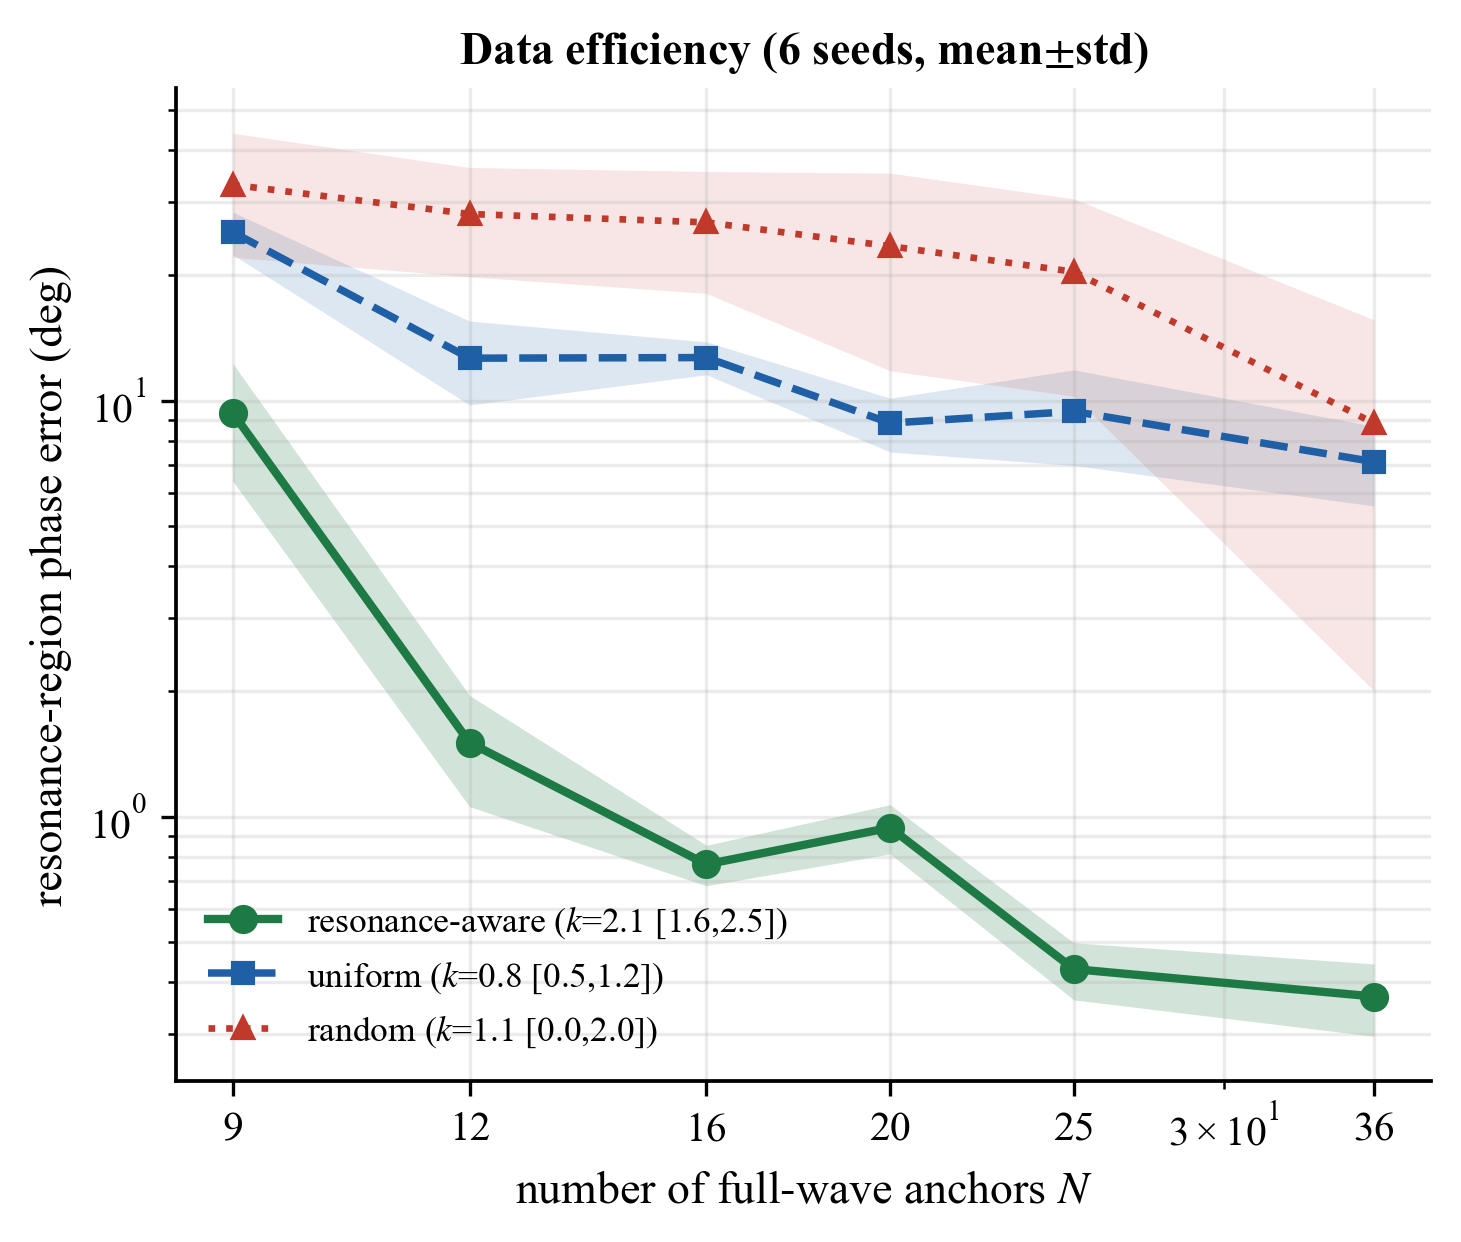
\includegraphics[width=0.62\linewidth]{fig_p3_scaling.png}
\caption{Data efficiency. Resonance-region phase error versus the number of full-wave anchors $N$ for
resonance-aware, uniform, and random ($\pm$std) placement. Resonance-aware sampling is uniformly best
and its error decays as $N^{-2.1}$ versus $N^{-0.8}$ (uniform) and $\approx\!N^{-1.1}$ (random; wide CI,
so we rely on per-budget dominance rather than exponent separation from random---see text).}
\label{fig:scaling}
\end{figure}

\paragraph{The acquisition criterion is deployable (no oracle), not an upper bound.} The curvature criterion above scores
candidates on the precomputed full-wave surface, so it measures the \emph{value of ideal placement}---an
upper bound, since a practitioner cannot score points they have not yet simulated. We therefore also run a fully
\emph{online} acquisition that may read the full-wave response \emph{only at anchors it has already
acquired}: starting from the four corners, it adds at each step the candidate of maximum committee
disagreement between a smooth and a sharp inverse-distance interpolant of the acquired complex
reflection. This data-driven uncertainty is large exactly where the \emph{observed} response is curved
(the resonance), and it is discoverable without the oracle. The online sampler retains most of the benefit
(Fig.~\ref{fig:acq}): its resonance-region exponent is $k\!=\!1.73\,[1.49,1.94]$---now statistically
separated from \emph{both} uniform ($0.82\,[0.68,0.97]$) and random ($0.84\,[0.59,1.31]$)---and it reaches
\SI{0.68}{\degree}$\pm$\SI{0.13}{\degree} resonance error at $N\!=\!36$ (oracle \SI{0.28}{\degree}, uniform
\SI{6.9}{\degree}, random \SI{8.6}{\degree}); at the smallest budgets it even matches the oracle on the
overall held-out surface. The data efficiency is thus a usable algorithm, deployable on a coarse pilot
acquisition, not a property of privileged access to the answer. (The committee powers were fixed a priori,
not tuned on the held-out outcome.) Finally, to confirm that this data efficiency is not an artefact of
selecting from the precomputed lattice, we re-ran the online sampler with openEMS \emph{in the loop} on a
continuous $41\times41$ candidate grid (\SI{0.1}{\milli\metre} spacing, far finer than the reference
lattice's \SI{0.4}{\milli\metre} in $L_y$ and \SI{0.5}{\milli\metre} in $L_x$), invoking the full-wave solver at each chosen continuous
$(L_x,L_y)$. Of the $20$ acquired anchors, $14$ fall strictly off the reference lattice; the surrogate
trained on them reaches \SI{1.42}{\degree} resonance-region phase error on the held-out $99$-point reference,
decaying monotonically from \SI{3.70}{\degree} at $N\!=\!9$ (\SI{2.92}{\degree}, \SI{1.81}{\degree},
\SI{1.42}{\degree} at $N\!=\!12,16,20$). The solver-in-the-loop sampler thus selects genuinely off-grid
geometries and still reaches sub-\SI{1.5}{\degree} accuracy on points it never queried, so the efficiency is
a property of the acquisition rule rather than of a privileged discrete pool. The run is taken to $N\!=\!20$
on this finer, harder continuous pool; the residual gap to the on-grid online figure (\SI{0.68}{\degree} at
$N\!=\!36$) reflects the smaller budget and the finer candidate set, and \SI{1.42}{\degree} is already well
inside design tolerance---this is a closure check, not a regression.

\paragraph{The advantage holds against principled active learning, not only uniform/random.} A natural
objection is that any sensible active-learning rule would do as well. It does not. We ran the textbook
information-theoretic baseline---Gaussian-process \emph{uncertainty} (maximum posterior-variance) sampling,
fit on the acquired anchors only---and it lands at \SI{5.56}{\degree} resonance error with exponent
$k\!=\!0.95\,[0.84,1.04]$ at $N\!=\!36$: barely better than uniform (\SI{6.9}{\degree}, $0.82$) and
$\sim\!20\times$ worse than the resonance-aware criterion (\SI{0.28}{\degree}, $k\!=\!2.26$, this comparison run).\footnote{The GP and LOLA--Voronoi benchmarks were re-run jointly with the resonance-aware criterion under one shared seed and configuration, so every rule is evaluated under identical conditions. The resonance-aware value in this joint comparison (\SI{0.28}{\degree}, $k\!=\!2.26$) differs from the headline data-efficiency run of Tables~\ref{tab:dataeff}--\ref{tab:scaling} (\SI{0.37}{\degree}, $k\!=\!2.07$) only through run-to-run seed/configuration variation, not through any re-tuning of the baselines.} The reason is
instructive: maximum-variance sampling \emph{space-fills}---it spreads points to reduce global
uncertainty---whereas a resonance-dominated response needs points \emph{crowded} into the narrow band where
the phase rotates. The curvature criterion is the principled choice here precisely because it targets that
band; off-the-shelf uncertainty sampling does not.

\paragraph{The advantage holds against a published adaptive sampler.} Uncertainty sampling is not the only
established alternative. We also benchmarked \emph{LOLA--Voronoi}~\cite{crombecq2011}, a widely used hybrid
sequential design that combines Voronoi-cell exploration with a local-nonlinearity (LOLA) exploitation
term---the standard published adaptive sampler for global surrogate modelling. Run on the same surface with
the same surrogate and budgets, it reaches \SI{2.61}{\degree} resonance-region error at $N\!=\!36$
($k\!=\!1.79\,[1.63,1.97]$): better than uniform, random, and GP uncertainty (its nonlinearity term does
pull some anchors toward the resonance), but still $\sim\!9\times$ worse than the oracle curvature criterion
(\SI{0.28}{\degree}, same comparison run) and $\sim\!4\times$ worse than the deployable online variant (\SI{0.68}{\degree}). The
reason is the same: LOLA--Voronoi spends half its budget on space-filling exploration, whereas a
resonance-dominated surface rewards crowding the narrow band. Across uniform, random, textbook GP
uncertainty, and a published adaptive sampler, the resonance-aware family is best at every budget
(Fig.~\ref{fig:acq})---the methodological point of the paper.

\begin{figure}[!htbp]\centering
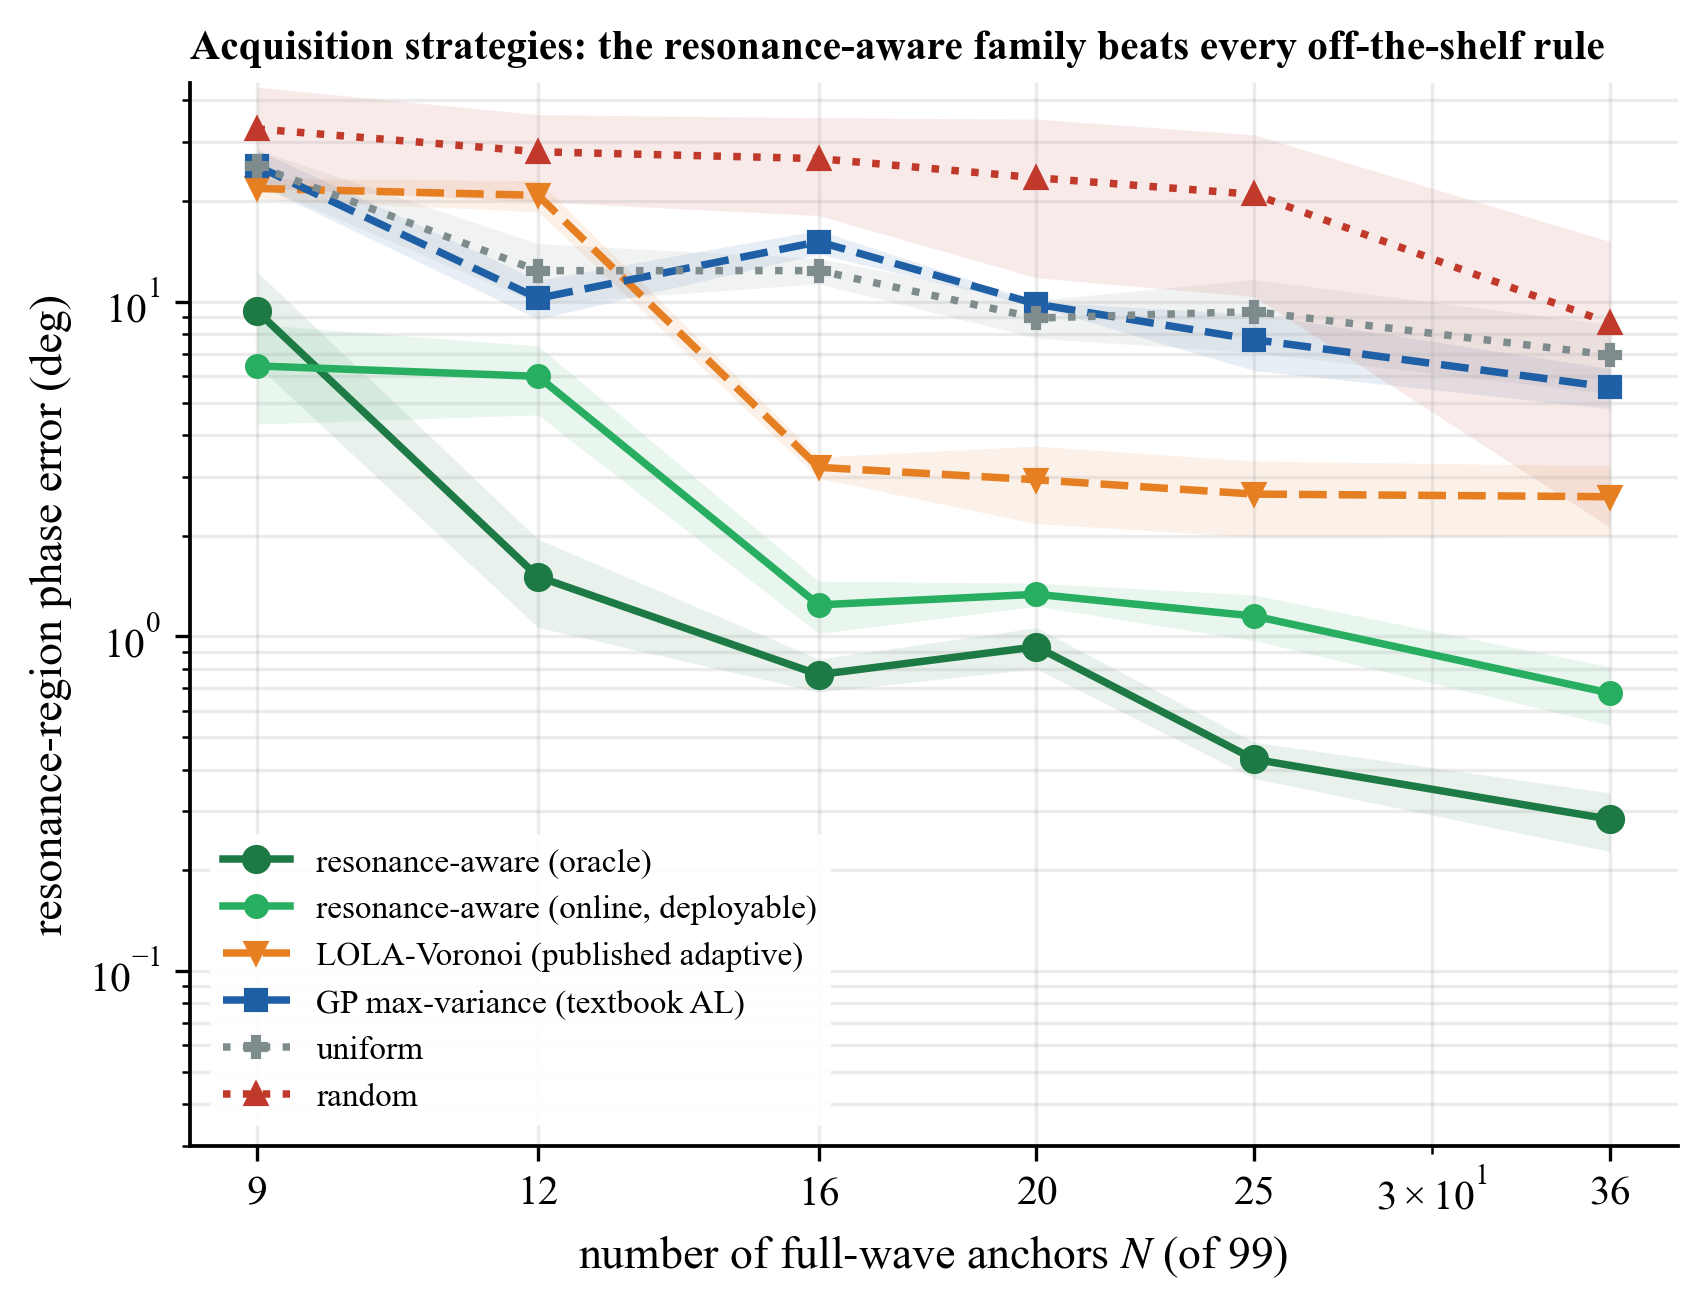
\includegraphics[width=0.7\linewidth]{fig_p3_acq.png}
\caption{Acquisition strategies on the 2-D patch (resonance-region phase error vs anchor budget, 6 seeds,
mean$\pm$std). The resonance-aware criterion (oracle) and its \emph{deployable} oracle-free online variant
are best at every budget; the published adaptive sampler LOLA--Voronoi~\cite{crombecq2011} and textbook
Gaussian-process maximum-variance sampling sit in between, and uniform/random are worst---because only a
resonance-\emph{targeted} rule crowds the narrow band where the design-relevant phase rotates. This is the
paper's methodological claim: a resonance-targeted acquisition beats every off-the-shelf rule we tested, and the
online variant delivers it without oracle access.}
\label{fig:acq}
\end{figure}

\begin{table}[!ht]\centering\small
\caption{Resonance-region phase error (deg, mean$\pm$std over 6 seeds) vs anchor budget $N$ for the three
placement strategies. Resonance-aware sampling is separated from uniform/random outside the error bars at
every $N$.}
\label{tab:dataeff}
\begin{tabular}{cccc}
\toprule
$N$ & uniform & random & resonance-aware \\
\midrule
9  & $25.4\pm3.0$ & $33.0\pm10.9$ & $\mathbf{9.35\pm2.94}$ \\
12 & $12.6\pm2.9$ & $28.1\pm8.2$  & $\mathbf{1.51\pm0.45}$ \\
16 & $12.7\pm1.2$ & $26.8\pm8.7$  & $\mathbf{0.77\pm0.09}$ \\
20 & $8.8\pm1.3$  & $23.5\pm11.7$ & $\mathbf{0.94\pm0.13}$ \\
25 & $9.4\pm2.4$  & $20.4\pm10.2$ & $\mathbf{0.43\pm0.07}$ \\
36 & $7.1\pm1.5$  & $8.8\pm6.8$   & $\mathbf{0.37\pm0.07}$ \\
\bottomrule
\end{tabular}
\end{table}

\begin{table}[!ht]\centering\small
\caption{Power-law exponent $k$ in $\varepsilon(N)=C\,N^{-k}$ (6 seeds; bootstrap 95\% CI). In the
resonance region the resonance-aware exponent is statistically separated from \emph{uniform}; its CI
overlaps \emph{random} only because the six-point random fit has a very wide CI, but random is dominated
outside the per-budget error bars at every $N$ (Table~\ref{tab:dataeff}). Over the whole surface the three
overlap (the resonance-aware advantage is then a lower constant, not a steeper exponent).}
\label{tab:scaling}
\begin{tabular}{lcc}
\toprule
strategy & held-out (overall) $k$ [95\% CI] & resonance region $k$ [95\% CI] \\
\midrule
uniform        & 0.98 [0.71, 1.27] & 0.83 [0.51, 1.15] \\
random         & 0.96 [0.02, 1.83] & 1.05 [0.03, 2.02] \\
resonance-aware& 1.12 [0.64, 1.75] & \textbf{2.07 [1.59, 2.50]} \\
\bottomrule
\end{tabular}
\end{table}

\section{Higher-dimensional generalization: a three-parameter cell}\label{sec:3d}
Does the data-efficiency advantage survive in higher dimension, where uniform sampling pays the curse of
dimensionality? We add a third geometry parameter, the substrate thickness $h$, and characterise the cell
by full wave over a $9\times9\times4=324$-point $(L_x,L_y,h)$ grid (phase span $344^\circ$, near-full
$360^\circ$ coverage). The resonance is a lower-dimensional manifold (small $L_y$) whose location drifts
with $h$, so a fixed $(L_x,L_y)$ no longer gives a fixed phase---a genuine three-way coupling.

The three-parameter study gives three findings (Table~\ref{tab:3d}, Fig.~\ref{fig:3d}). First, the curvature criterion of
Section~\ref{sec:method}, applied \emph{globally} in 3-D---the unchanged 2-D method, our honest baseline,
not a constructed foil---\emph{fails}: it over-concentrates anchors on
the resonance of a single $h$-slice and never learns the $h$-dependence (resonance error stuck at
$38$--$59^\circ$, not improving with $N$; Table~\ref{tab:3d}, last column). The remedy is to
\emph{stratify} the acquisition along the added axis---cover the resonance band within every $h$-slice.
With stratified resonance-aware sampling the advantage not only carries but \emph{widens}: resonance-region
error falls to \SI{10.0}{\degree} at $N\!=\!30$ and \SI{0.6}{\degree} at $N\!=\!120$, whereas uniform never
falls below $\approx\!\SI{18}{\degree}$ at any tested budget and random needs $N\!=\!120$ (\SI{4.5}{\degree})
to approach what stratified sampling already reaches at $N\!=\!60$ (\SI{2.9}{\degree})---a $\approx\!2\times$
anchor saving over the best non-resonance-aware strategy.

Second, the decay rates separate cleanly. A power-law fit $\varepsilon_\mathrm{res}\propto N^{-k}$
(2000-sample bootstrap) gives $k=2.38$ (95\% CI $[2.29,2.50]$, $r^2=0.98$) for stratified resonance-aware
sampling, versus $k=0.50$ $[0.46,0.55]$ for uniform and $k=1.30$ $[1.13,1.55]$ for random; the confidence
intervals do not overlap, so the steeper convergence is statistically resolved rather than a seed artefact.
The curse of dimensionality is then explicit. To reach a common resonance target ($\le\!7^\circ$), the
resonance-region anchor saving of resonance-aware over uniform sampling grows from $\approx\!2.1\times$ in
2-D to \emph{unbounded} in 3-D: uniform's resonance-error floor rises from $\approx\!7^\circ$ (2-D) to
$\approx\!18^\circ$ (3-D)---it never reaches the target---while stratified resonance-aware sampling holds a
sub-degree floor ($0.59^\circ$ in 3-D, $0.37^\circ$ in 2-D). On the \emph{whole} surface (a less
design-relevant metric) the saving still grows, from $\approx\!1.1\times$ to $\approx\!2.0\times$. The
lesson is concrete and transferable: in higher dimension, active sampling must be stratified along the
added axes; done so, the full-wave-budget saving \emph{grows}, because uniform coverage becomes
exponentially expensive while the resonance stays low-dimensional. (On the whole surface, random and
uniform remain competitive---resonance-aware specialises in the resonant phase, which is exactly the
quantity coded designs need.)

Third, the 3-D advantage is carried by the \emph{sampling}, not the model: at $N\!=\!120$ stratified
anchors the differentiable MLP attains \SI{0.42}{\degree} resonance error, Gaussian-process kriging
\SI{0.58}{\degree}, and RBF interpolation \SI{4.93}{\degree}---the neural and GP surrogates remain an order
of magnitude tighter than RBF on the same anchors, mirroring the 2-D comparison of Section~\ref{sec:base}.

\begin{table}[!ht]\centering\small
\caption{Three-parameter cell: resonance-region phase error (deg, mean$\pm$std, 5 seeds) vs anchor budget
$N$ (of 324). The naive global criterion fails (stuck $38$--$59^\circ$); \emph{$h$-stratified}
resonance-aware sampling dominates and widens its lead---uniform never reaches the accuracy it attains.}
\label{tab:3d}
\begin{tabular}{ccccc}
\toprule
$N$ & uniform & random & resonance-aware ($h$-stratified) & naive (global) \\
\midrule
20  & $43.8\pm0.8$ & $49.7\pm10.4$ & $\mathbf{41.0\pm2.9}$ & $59.1$ \\
30  & $37.1\pm1.1$ & $46.7\pm7.4$  & $\mathbf{10.0\pm1.3}$ & $45.8$ \\
45  & $36.1\pm0.6$ & $32.2\pm6.0$  & $\mathbf{7.0\pm0.8}$  & $37.7$ \\
60  & $27.5\pm0.9$ & $25.4\pm10.6$ & $\mathbf{2.9\pm0.5}$  & $38.2$ \\
90  & $18.3\pm1.3$ & $11.2\pm4.9$  & $\mathbf{0.8\pm0.1}$  & $42.4$ \\
120 & $20.0\pm1.8$ & $4.5\pm2.6$   & $\mathbf{0.6\pm0.3}$  & $45.3$ \\
\bottomrule
\end{tabular}
\end{table}

\begin{figure}[!htbp]\centering
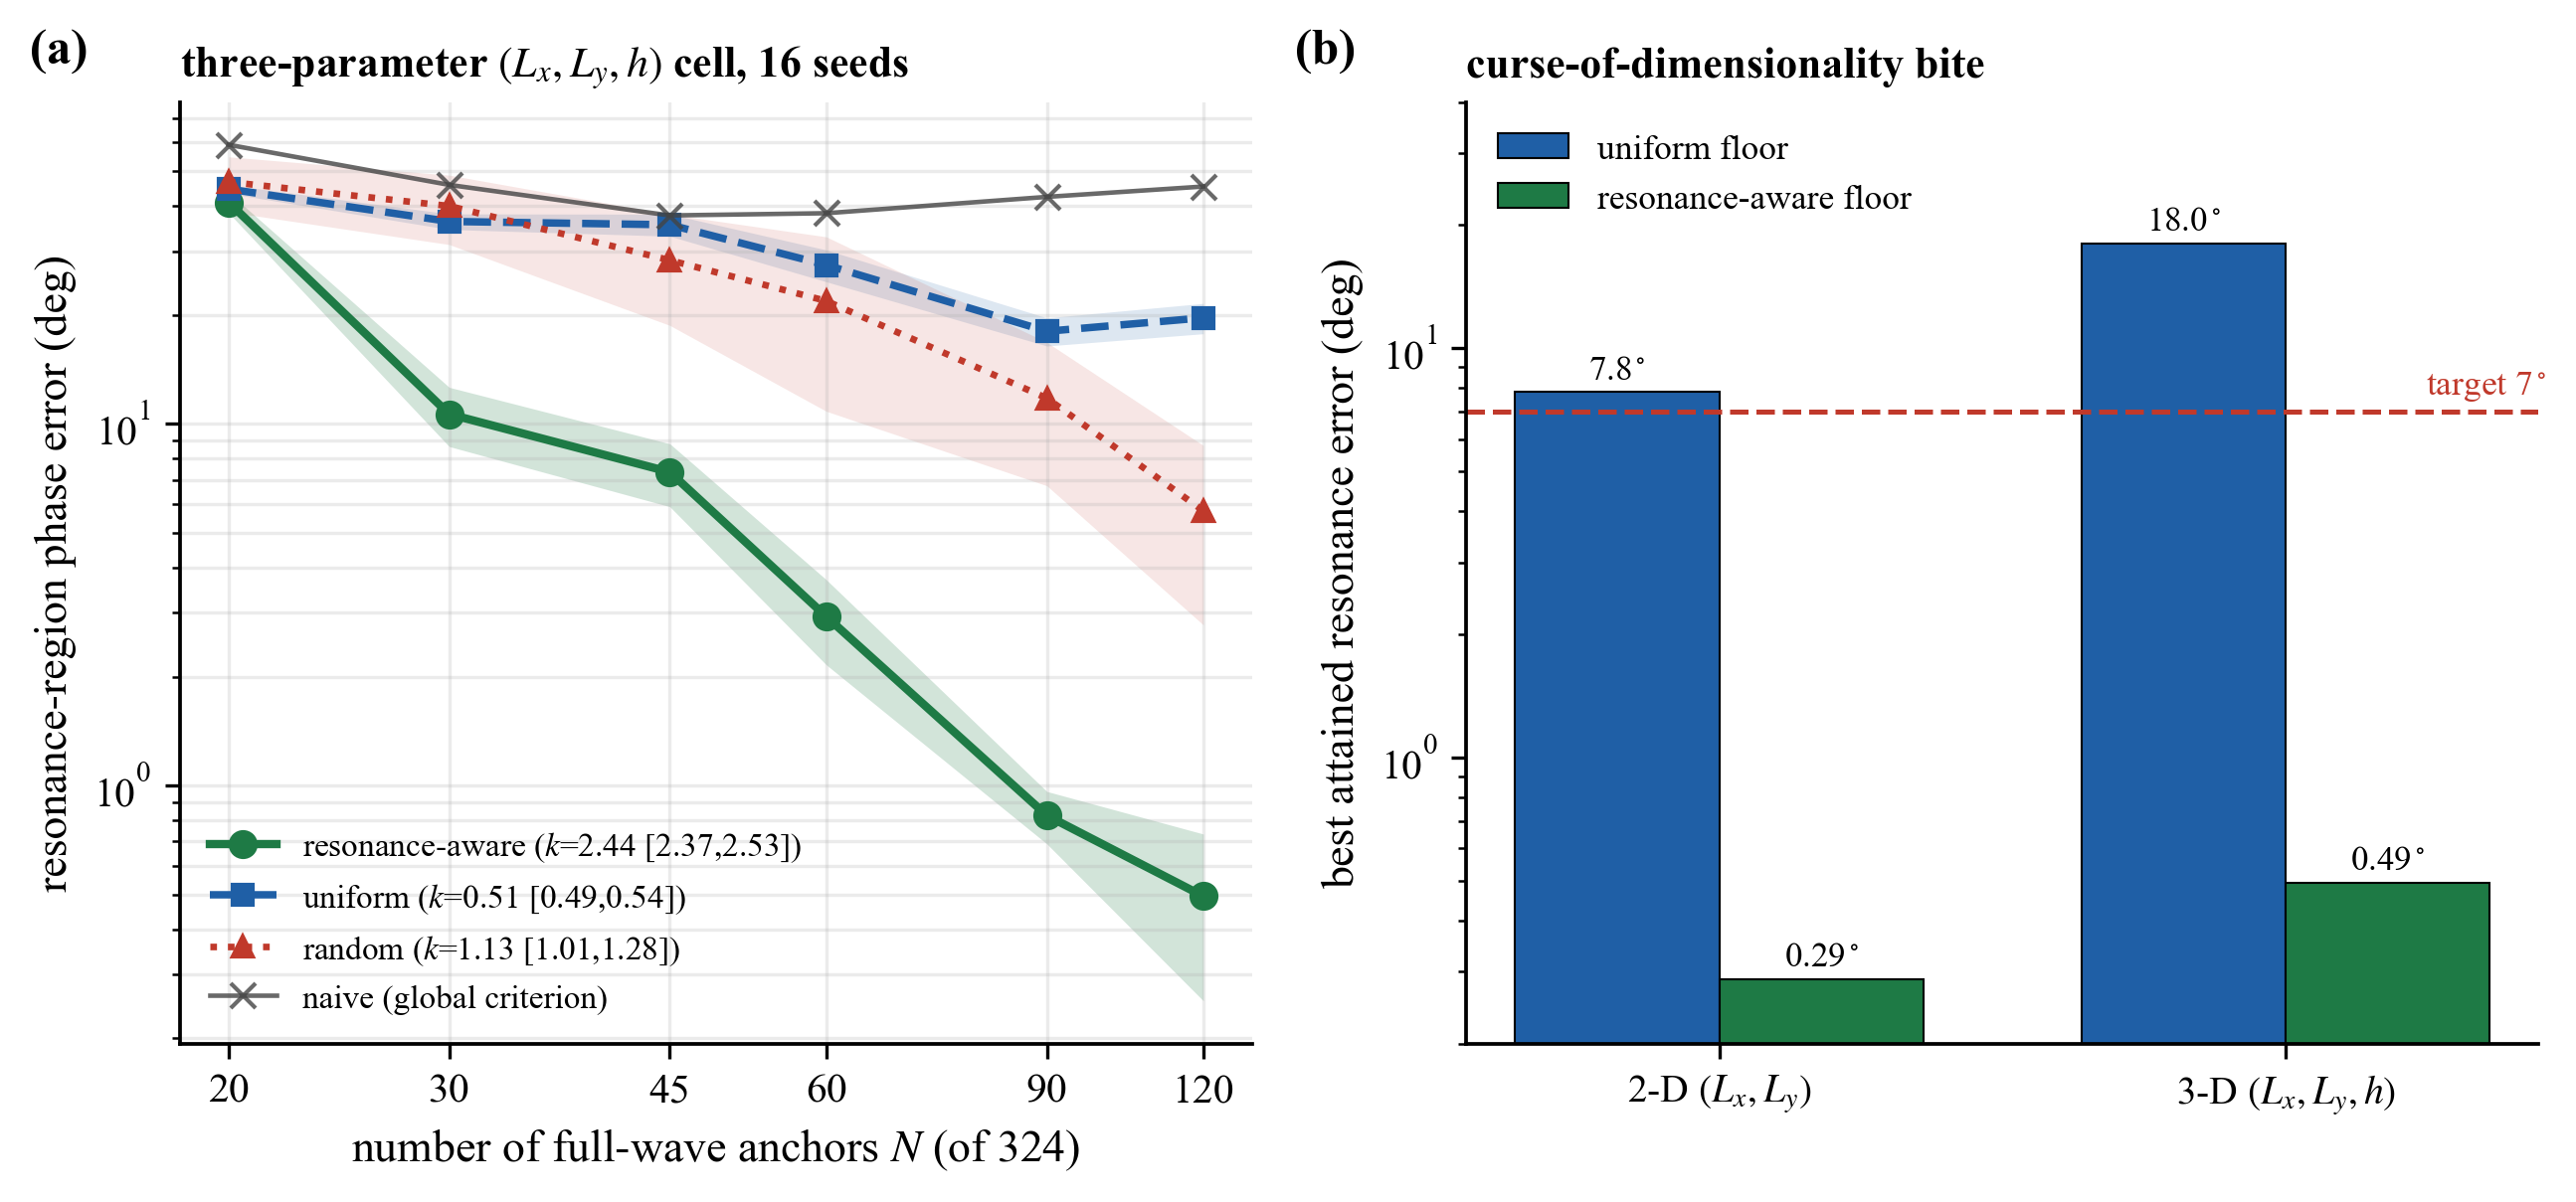
\includegraphics[width=\linewidth]{fig_p3_3d.png}
\caption{Three-parameter $(L_x,L_y,h)$ cell (5 seeds, mean$\pm$std). \textbf{(a)} Resonance-region phase
error vs anchor budget $N$: $h$-stratified resonance-aware sampling dominates with the steepest decay
exponent ($k\!=\!2.38$, non-overlapping bootstrap CI), while the naive global criterion stalls.
\textbf{(b)} Curse-of-dimensionality bite: the best resonance error uniform sampling attains rises from
$\approx\!7^\circ$ (2-D) to $\approx\!18^\circ$ (3-D), crossing above the $7^\circ$ target it once met,
whereas stratified resonance-aware sampling holds a sub-degree floor in both---so the full-wave-budget
saving \emph{widens} with dimension.}
\label{fig:3d}
\end{figure}

\section{Transferring the surrogate across substrates}\label{sec:transfer}
A surrogate is most useful if it need not be rebuilt from scratch whenever a design parameter outside the
swept set changes. We test this directly. We pretrain the surrogate on one substrate (condition~A, FR4
thickness $h\!=\!\SI{1.0}{mm}$) over its full $(L_x,L_y)$ surface, then \emph{adapt} it to a different
substrate (condition~B, $h\!=\!\SI{1.5}{mm}$, generated by an independent openEMS sweep; the thicker board
shifts the resonance) by \emph{warm-starting} from the condition-A weights and fine-tuning on only a
handful of new condition-B anchors. We compare warm-start against training from scratch on the
\emph{same} new anchors with the \emph{same} optimiser budget---so the only difference is the
initialisation (Fig.~\ref{fig:transfer}, resonance-aware anchors on B, 6 seeds).

Transfer is decisive. Warm-start reaches \SI{3.7}{\degree} resonance-region error from just $k\!=\!4$ new
full-wave anchors and stays in the \SIrange{3.5}{5}{\degree} band thereafter, whereas training from scratch
is erratic and needs $k\!=\!16$ anchors merely to reach \SI{6.2}{\degree}; at every budget warm-start is
$1.2$--$8.5\times$ more accurate, and warm-start at $k\!=\!4$ already \emph{beats} scratch at $k\!=\!16$.
The surrogate therefore transfers: the $(L_x,L_y)\!\to\!\Gamma$ structure learned on one board is reused,
so adapting to a new substrate costs $\sim\!4\times$ fewer full-wave simulations than starting over. This
``train once, adapt cheaply'' behaviour is the practical pay-off of a lightweight, data-driven surrogate;
we demonstrate it for a substrate-thickness change and do not claim it across arbitrarily different cells.

\begin{figure}[!htbp]\centering
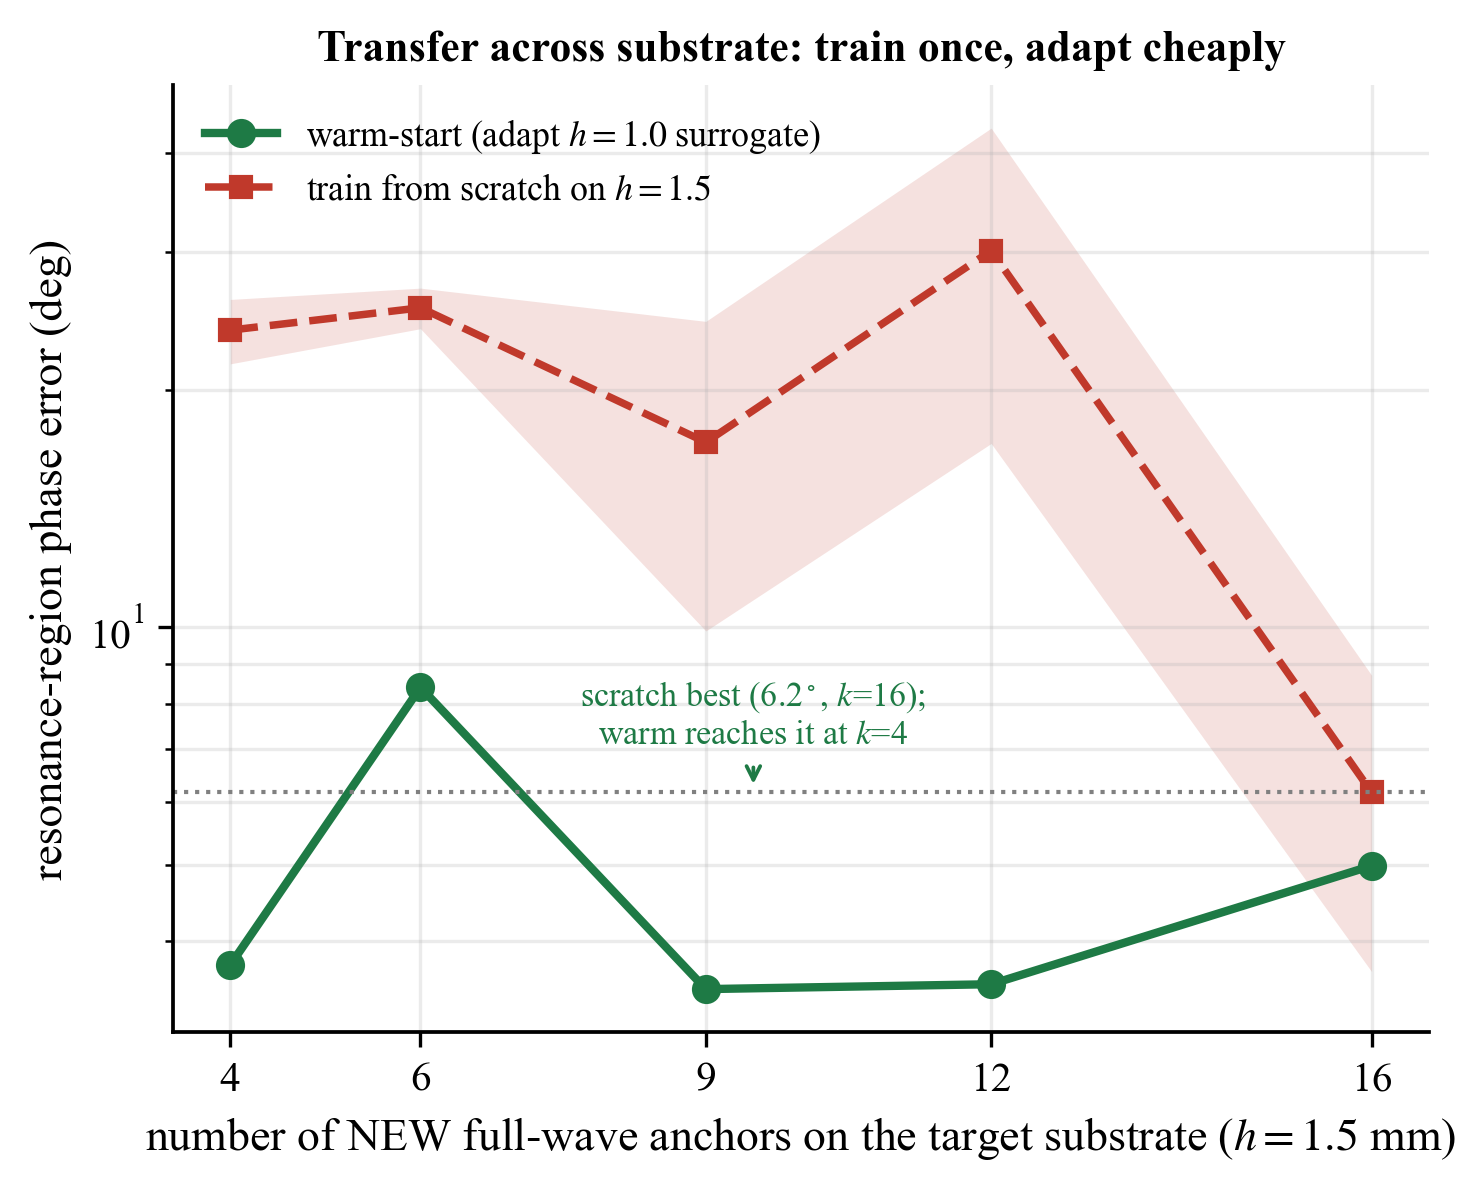
\includegraphics[width=0.6\linewidth]{fig_p3_transfer.png}
\caption{Transfer across substrate thickness. Warm-starting the $h\!=\!\SI{1.0}{mm}$ surrogate and
fine-tuning on a few $h\!=\!\SI{1.5}{mm}$ anchors reaches low resonance error from $k\!=\!4$ anchors;
training from scratch needs $k\!=\!16$ to match---$\sim\!4\times$ fewer full-wave simulations to retarget a
new substrate (6 seeds, mean$\pm$std).}
\label{fig:transfer}
\end{figure}

\section{The advantage recurs on further cell topologies}\label{sec:topology}
Is the active-sampling advantage specific to the rectangular patch, or a property of the \emph{method}? We
repeat the 2-D study on two structurally different elements, both characterised by the same openEMS
waveguide-simulator sweep (99-point grid).

\paragraph{A cross dipole (single resonance).} The first element is a \emph{cross dipole} (two crossed
strips, arm lengths $L_x,L_y$, width \SI{0.5}{mm}; phase span $320^\circ$), where the resonance comes from
the $E$-aligned arm rather than a patch edge. The advantage recurs and \emph{sharpens}
(Fig.~\ref{fig:cross}a): resonance-aware sampling reaches \SI{1.43}{\degree} at $N\!=\!36$
($k\!=\!1.70\,[1.44,1.95]$), while uniform sampling \emph{fails outright}---it never improves with budget
($k\!=\!-0.07\,[-0.18,0.05]$, stuck at $40$--$54^\circ$), because a uniform grid almost never lands on the
narrow resonant arm---and random reaches only \SI{13.1}{\degree} ($k\!=\!1.06$). The resonance-aware
exponent is separated from \emph{both} baselines.

\paragraph{A dual-resonance cell (two bands).} The second element is a \emph{dual-resonance} cell---two
separated $y$-dipoles whose lengths are the two swept parameters, giving \emph{two} resonance ridges
(phase span $354^\circ$). This is a harder test: the acquisition must concentrate on \emph{both} bands. The
advantage still recurs, though more modestly (Fig.~\ref{fig:cross}b): resonance-aware reaches
\SI{18.5}{\degree} at $N\!=\!36$ ($k\!=\!0.65\,[0.57,0.74]$) versus \SI{45}{\degree} (uniform,
$k\!=\!0.16$) and \SI{34}{\degree} (random, $k\!=\!0.25$)---about $2\times$ more accurate with a steeper
exponent. We report honestly that \emph{no} method reaches sub-degree error here: resolving two narrow
bands needs more than the $\le\!36$-anchor budget that suffices for a single band, an expected
budget-versus-band-count limit. The comparative ranking, however, is unchanged---the curvature criterion
again dominates.

Across the patch, the cross dipole (where uniform collapses), and the dual-resonance cell (the harder
two-band case), the same curvature-driven acquisition wins. This is consistent with the data-efficiency
advantage being a property of the acquisition criterion rather than of one cell shape. These are still
planar cells in one solver; a non-planar or measured element is the natural next test.

\begin{figure}[!htbp]\centering
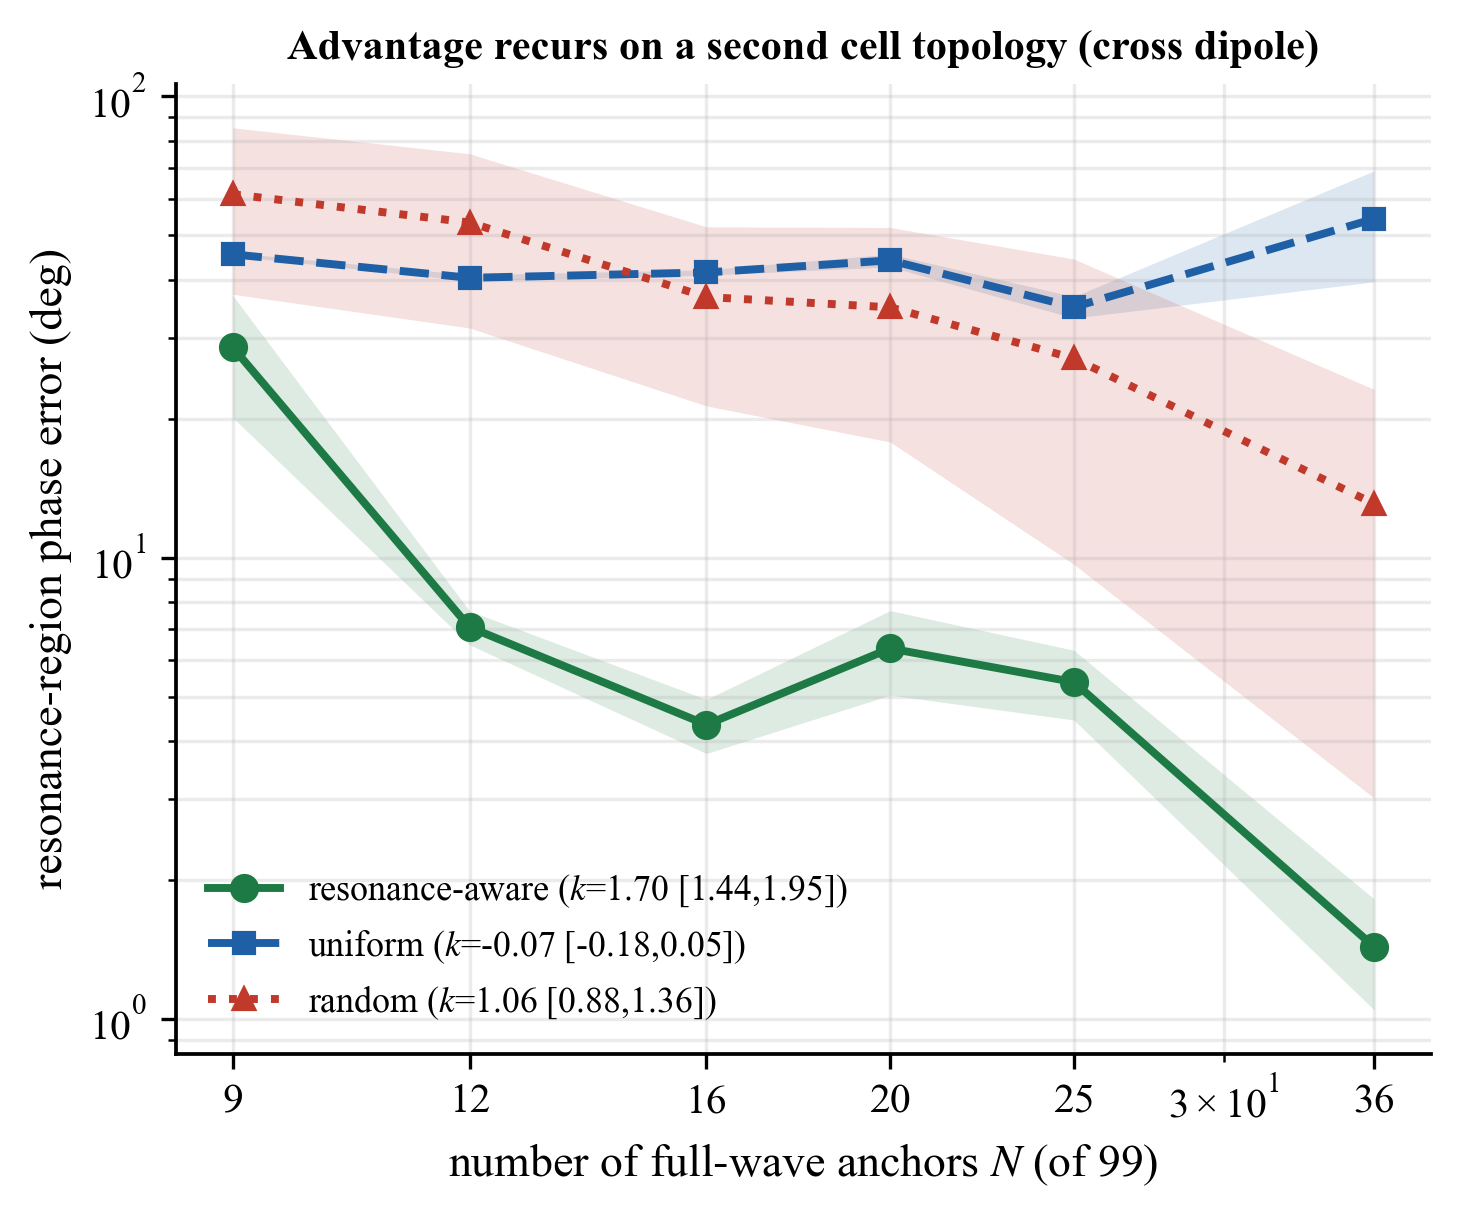
\includegraphics[width=\linewidth]{fig_p3_cross.png}
\caption{The resonance-aware advantage recurs on two further cell topologies (resonance-region error vs
anchor budget, 6 seeds, mean$\pm$std). \textbf{(a)} Cross dipole (single resonance): resonance-aware
($k\!=\!1.70$) reaches \SI{1.43}{\degree} at $N\!=\!36$ while uniform fails entirely ($k\!\approx\!0$,
$\sim\!54^\circ$). \textbf{(b)} Dual-resonance cell (two bands): the advantage recurs more modestly---
resonance-aware (\SI{18.5}{\degree}, $k\!=\!0.65$) is $\sim\!2\times$ better than uniform/random, but no
method reaches sub-degree because resolving two narrow bands needs more anchors. The comparative ranking is
unchanged across all cells.}
\label{fig:cross}
\end{figure}

\section{The method transfers off the electromagnetic testbed: two non-EM resonances}\label{sec:outdomain}
The criterion is claimed to target \emph{any} expensive-to-sample, resonance-dominated response, not just
reflectarray cells. We test that claim directly by running the \emph{identical} pipeline---the same
differentiable surrogate (Section~\ref{sec:method}), the same curvature acquisition (Eq.~\eqref{eq:acq},
Algorithm~\ref{alg:active}), the same uniform/random baselines, and the same bootstrap exponent---on two
textbook \emph{non-electromagnetic} resonance-dominated responses, changing \emph{only the oracle}. Each is
a two-parameter complex response on a $99$-point grid, with a sharp resonance localised in a narrow band of
one parameter and sharpening along the other, so the regime matches the one the method targets (a localised
high-$Q$ feature on a smooth plateau).
(i) A \emph{driven damped oscillator / series-RLC} response, the Lorentzian $H=1/(\delta+\im)$ with reduced
detuning $\delta$ set by the two design parameters---$|H|$ peaks and the phase swings through resonance.
(ii) A \emph{Fano resonance} line shape $t=(\delta+q)/(\delta+\im)$ ($q=1.5$), the asymmetric profile
ubiquitous in optics and condensed matter.

The advantage transfers (Fig.~\ref{fig:outdomain}). On the RLC/oscillator response, resonance-aware sampling
reaches \SI{0.41}{\degree} resonance-region error at $N\!=\!36$ with exponent $k\!=\!2.48\,[2.32,2.71]$,
statistically separated from uniform (\SI{4.64}{\degree}, $k\!=\!0.62\,[0.38,0.78]$) and best at every
budget. On the Fano line shape the contrast is starker, mirroring the cross dipole: uniform sampling
\emph{fails outright}---it never resolves the asymmetric resonance, stalling at $\approx\!\SI{35}{\degree}$
($k\!=\!0.17\,[0.15,0.19]$)---whereas resonance-aware sampling reaches sub-degree (\SI{0.55}{\degree}) once
it has enough anchors to locate the narrow band. (We report honestly that on the very sharp Fano profile even
resonance-aware sampling needs $N\!\gtrsim\!20$ before it locks onto the band; below that it has not yet
found the resonance, a threshold the smooth-plateau-dominated uniform grid never crosses at all.)

These two systems are \emph{analytic}, so their oracle is cheap; this experiment therefore demonstrates that
the \emph{acquisition criterion} transfers to non-electromagnetic resonance-dominated responses, not that it
saves cost on an expensive non-EM solver. With that caveat, the data-efficiency advantage now recurs across
three electromagnetic cell topologies (patch, cross dipole, dual-resonance) \emph{and} two non-electromagnetic
line shapes (driven-oscillator/RLC, Fano), changing only the oracle---consistent with the advantage being a
property of the resonance-aware acquisition criterion for this class of responses, as claimed, rather than
of electromagnetics.

\begin{figure}[!htbp]\centering
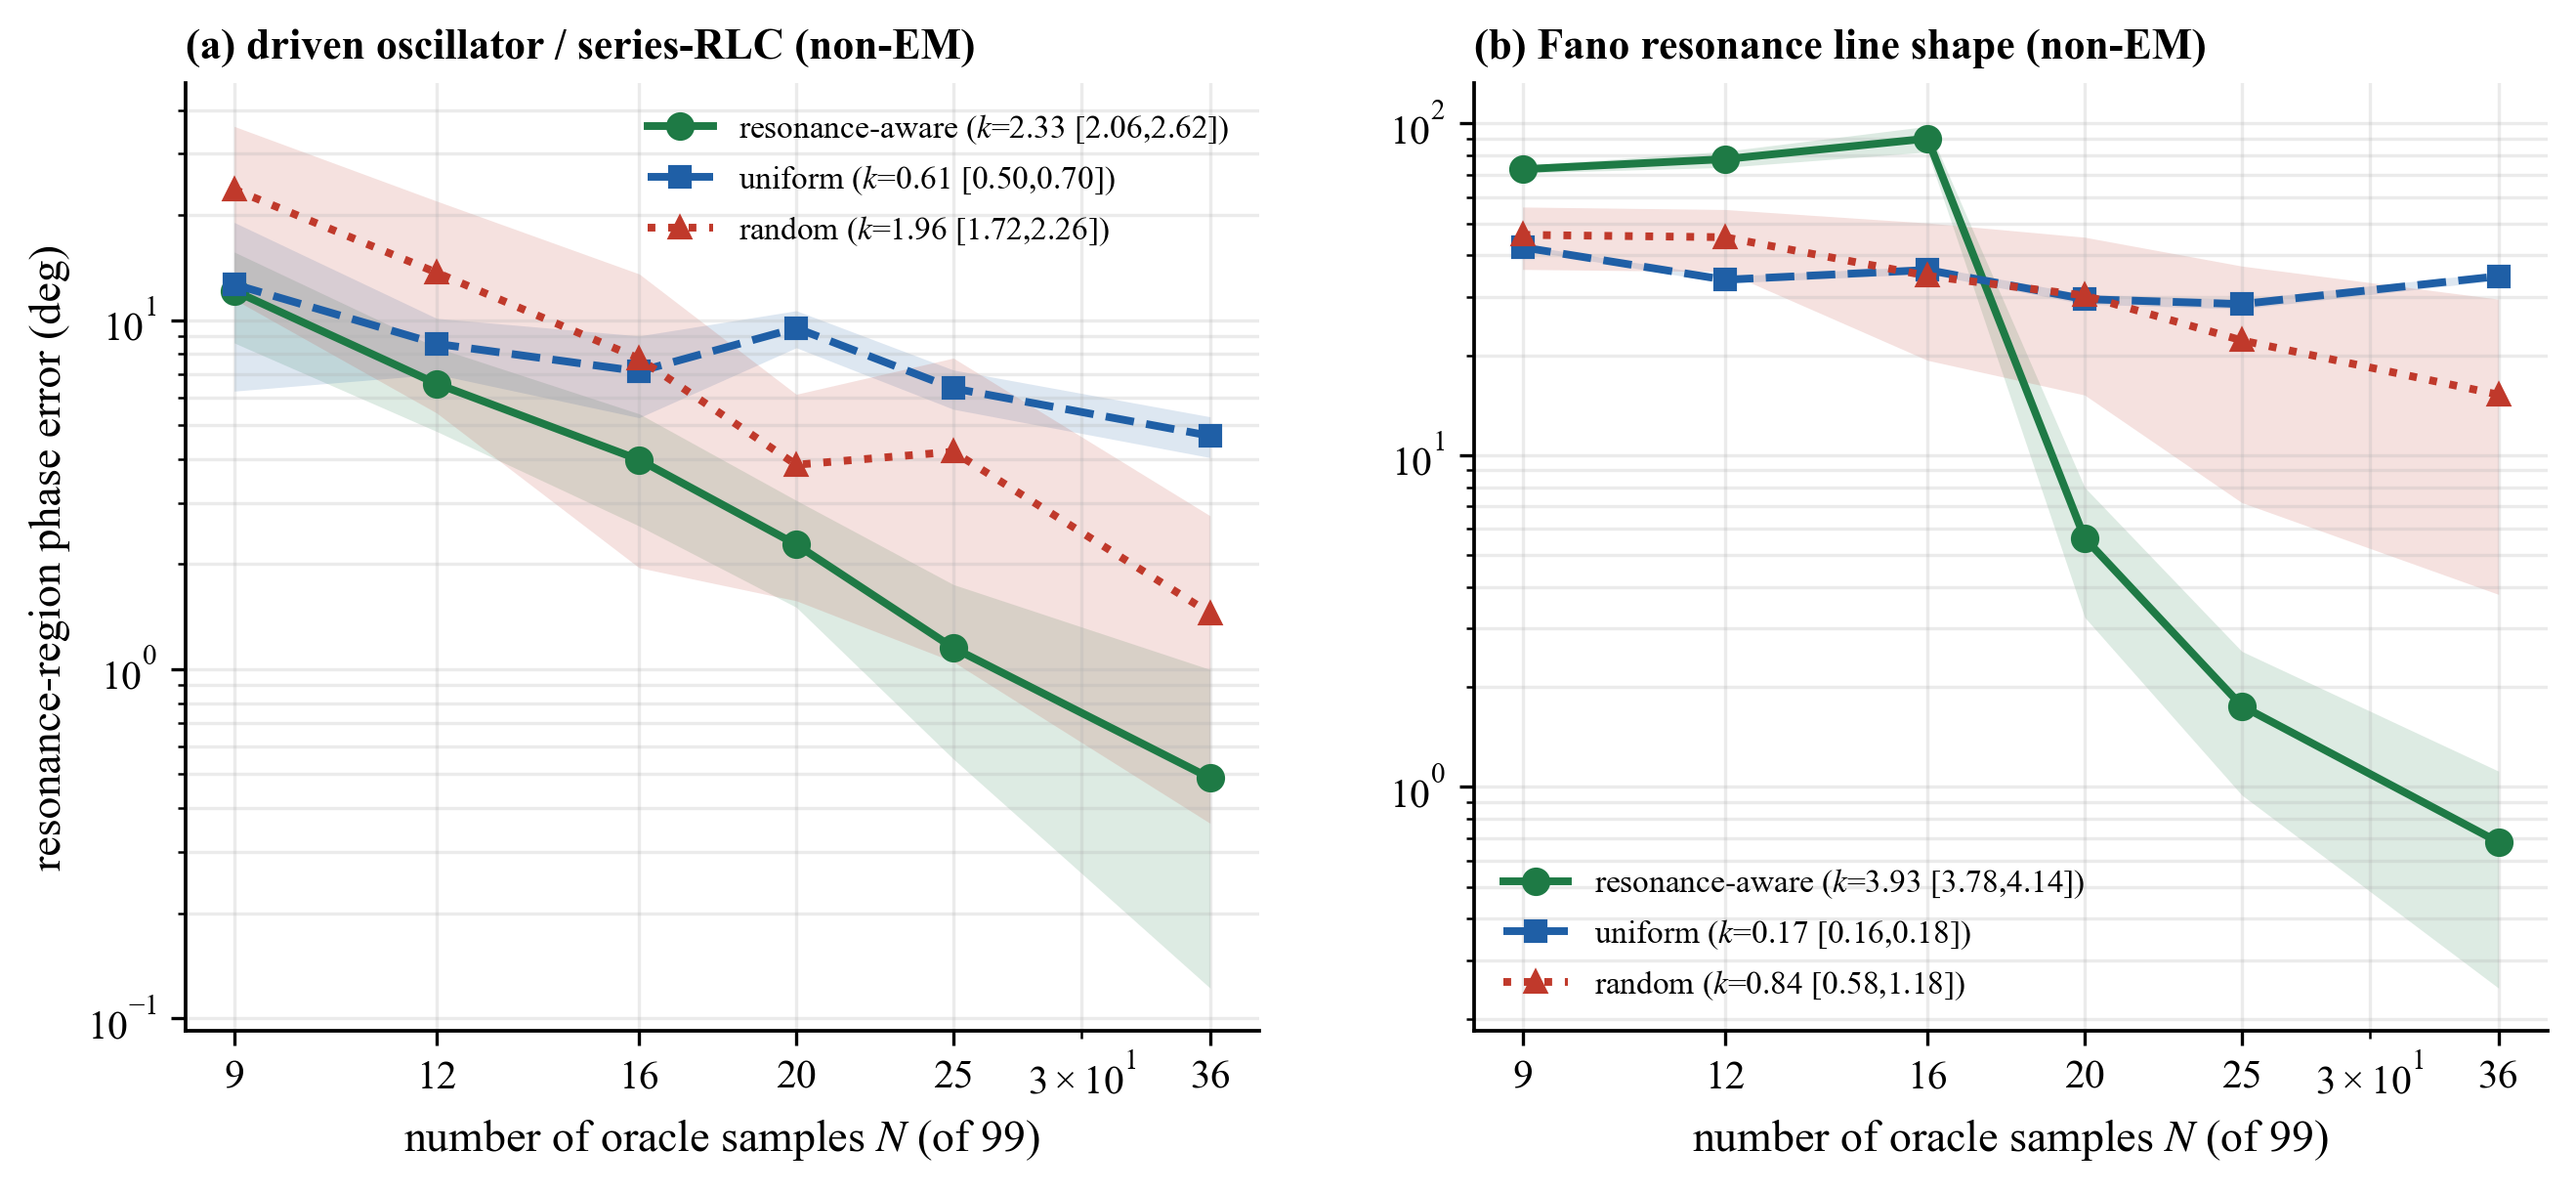
\includegraphics[width=\linewidth]{fig_p3_outdomain.png}
\caption{The same resonance-aware criterion, applied to two \emph{non-electromagnetic} resonance-dominated
responses (resonance-region phase error vs oracle samples, 6 seeds, mean$\pm$std; only the oracle physics
changed). \textbf{(a)} Driven oscillator / series-RLC (Lorentzian): resonance-aware ($k\!=\!2.48$) reaches
\SI{0.41}{\degree} at $N\!=\!36$, separated from uniform ($k\!=\!0.62$) and best at every budget.
\textbf{(b)} Fano resonance: uniform fails entirely (stuck $\approx\!\SI{35}{\degree}$, $k\!\approx\!0.17$),
while resonance-aware reaches sub-degree once it locates the narrow band---a non-EM analogue of the cross
dipole. The advantage is a property of the acquisition criterion, not of electromagnetics.}
\label{fig:outdomain}
\end{figure}

\section{Comparison with standard surrogates}\label{sec:base}
At equal anchor budgets the differentiable MLP surrogate matches or beats the baselines
(Fig.~\ref{fig:eval}a). On \emph{uniform} anchors all three are comparable---at $N\!=\!36$ the phase MAE
is \SI{1.84}{\degree} (MLP), \SI{2.02}{\degree} (SVR) and \SI{2.30}{\degree} (ANN)---so a published-style
support-vector surrogate is on par when the data are well spread, and we say so plainly. The difference
emerges under the \emph{clustered} resonance-aware anchors: the RBF support-vector regressor degrades
markedly (MAE $>\SI{14}{\degree}$) because kernel regression with a single global length scale and
non-uniform support extrapolates poorly across the resonance, and the plain ANN is competitive only at
the largest budget. The differentiable network is thus the better partner for resonance-aware
sampling---which is precisely the regime that minimises full-wave cost---giving phase MAE
\SI{1.84}{\degree} ($N\!=\!16$) and \SI{1.12}{\degree} ($N\!=\!36$) on those anchors. The practical
implication is that the sampling strategy and the learner must be chosen together: active sampling pays
off only with a learner that tolerates clustered training points.

One might object that a 2-parameter surface needs no neural model at all---a classical interpolant would
do. We therefore add thin-plate-spline RBF interpolation and Gaussian-process kriging on the same anchors.
The differentiable MLP is best at every budget: on resonance-aware anchors at $N\!=\!16$ it gives
\SI{1.84}{\degree} versus \SI{6.33}{\degree} (RBF) and \SI{19.4}{\degree} (kriging), and at $N\!=\!36$
\SI{1.11}{\degree} versus \SI{1.47}{\degree} and \SI{5.85}{\degree}. The classical interpolants suffer the
\emph{same} clustered-anchor pathology as the SVR---kriging in particular, with a single global length
scale---so the neural surrogate is not a gratuitous choice: it is the model that best exploits the
resonance-aware anchors while still providing autodiff geometry gradients (Table~\ref{tab:baseline},
Fig.~\ref{fig:baseline2}).

\begin{table}[!ht]\centering\small
\caption{Held-out phase MAE (deg) vs the differentiable MLP, RBF interpolation, and Gaussian-process
kriging, at matched anchor budgets. The MLP is best at every budget; the classical interpolants suffer
the same clustered-anchor pathology as the SVR (kriging worst), justifying the neural surrogate.}
\label{tab:baseline}
\begin{tabular}{lccc}
\toprule
$N$ (strategy) & MLP & RBF interp.\ & GP kriging \\
\midrule
9 (uniform)          & \textbf{9.16} & 15.55 & 17.63 \\
9 (resonance-aware)  & \textbf{4.18} & 14.47 & 16.58 \\
16 (uniform)         & \textbf{4.15} & 7.68  & 8.34 \\
16 (resonance-aware) & \textbf{1.84} & 6.33  & 19.36 \\
25 (uniform)         & \textbf{2.07} & 3.04  & 4.52 \\
25 (resonance-aware) & \textbf{1.47} & 4.31  & 8.62 \\
36 (uniform)         & \textbf{1.84} & 2.88  & 3.94 \\
36 (resonance-aware) & \textbf{1.11} & 1.47  & 5.85 \\
\bottomrule
\end{tabular}
\end{table}

\begin{figure}[!htbp]\centering
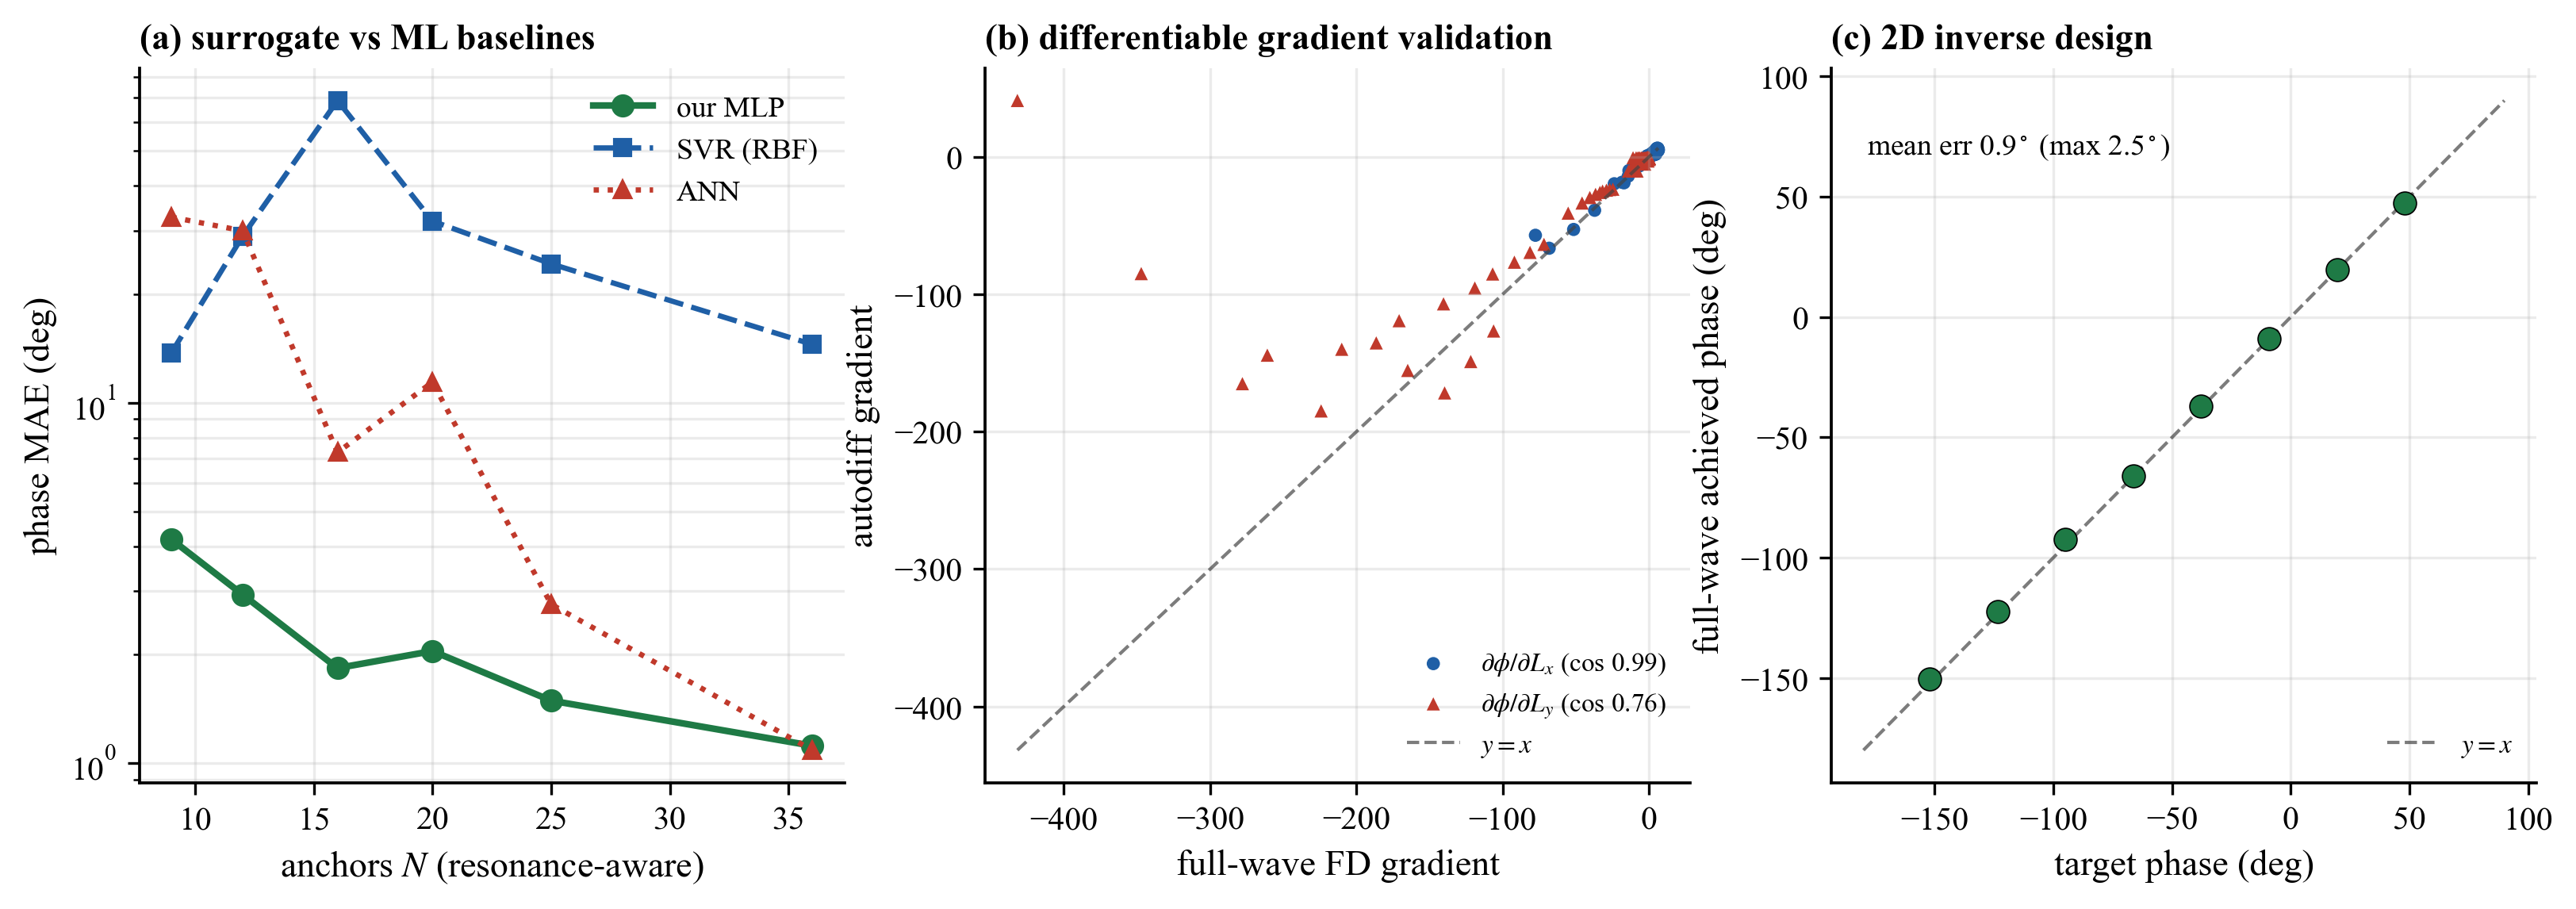
\includegraphics[width=0.99\linewidth]{fig_p3_eval.png}
\caption{(a) At equal anchor budgets (resonance-aware), the differentiable MLP surrogate matches or
beats SVR and ANN baselines (phase MAE, log scale). (b) Autodiff geometry gradient versus full-wave
finite difference: the transverse partial $\partial\angle\Gamma/\partial L_x$ is highly consistent
(cosine $0.99$) and the sharper resonant partial $\partial\angle\Gamma/\partial L_y$ moderately so
(cosine $0.76$; a fine $\pm\SI{0.1}{mm}$ full-wave check, Table~\ref{tab:finefd}, shows this is a
coarse-reference artefact). (c) Two-parameter inverse design: full-wave-verified achieved phase versus target for
eight goals (mean error \SI{0.9}{\degree}).}
\label{fig:eval}
\end{figure}

\begin{figure}[!htbp]\centering
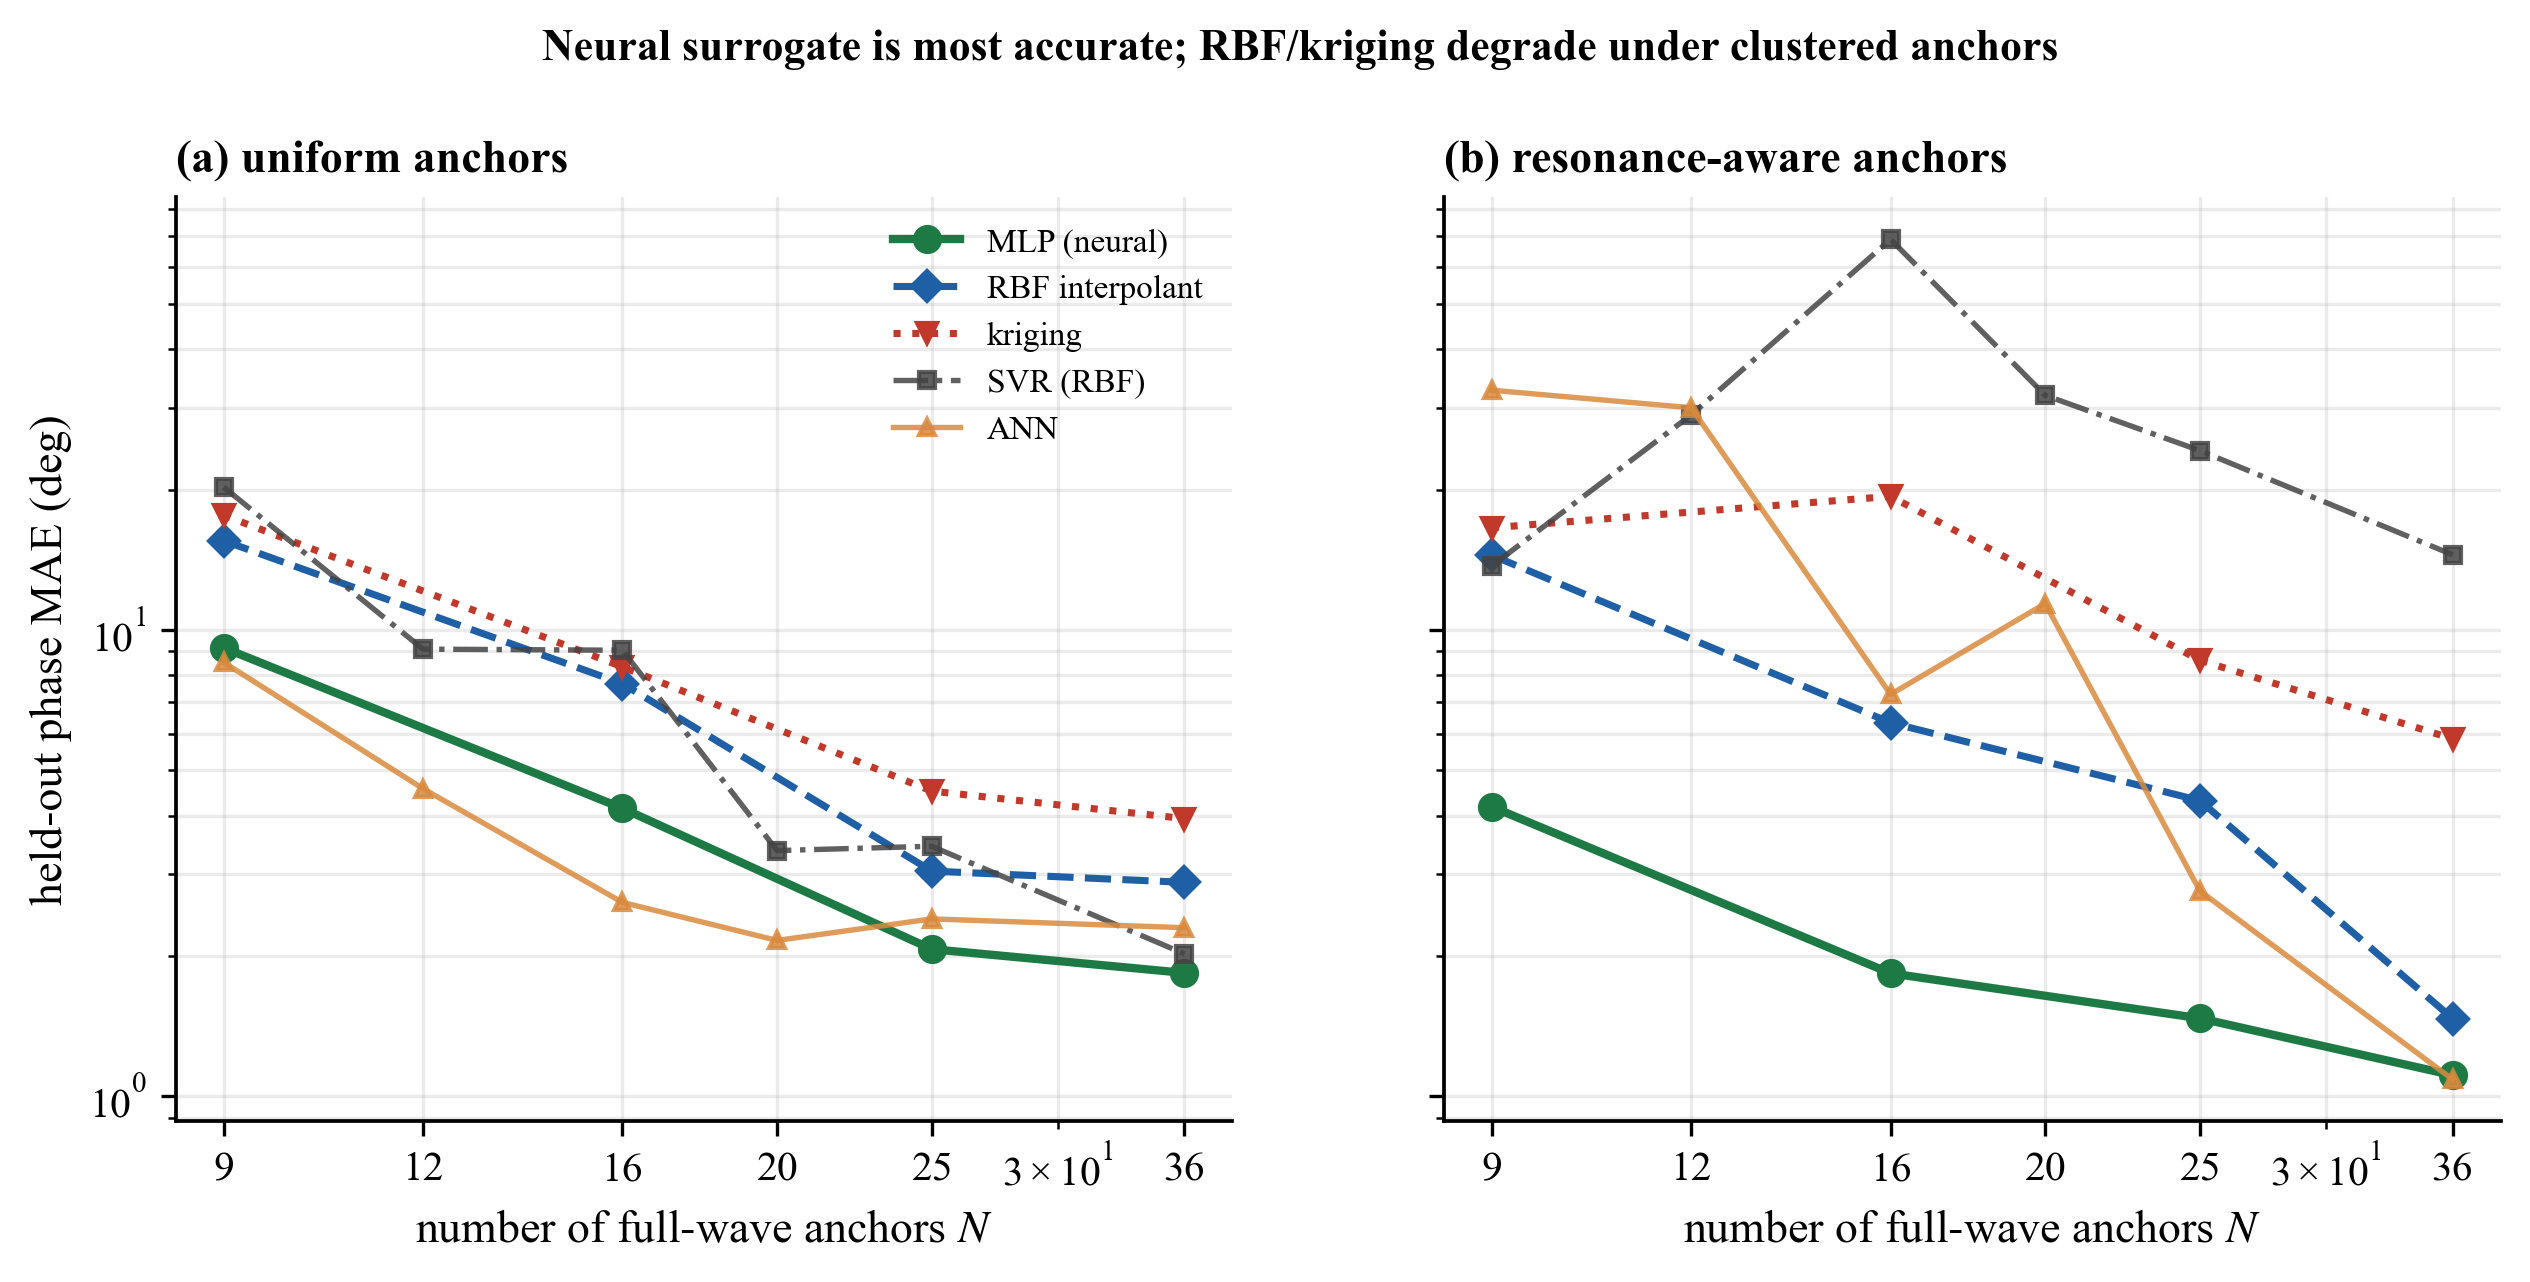
\includegraphics[width=0.99\linewidth]{fig_p3_baseline2.png}
\caption{The neural surrogate justified. Held-out phase MAE vs $N$ for the MLP, SVR, ANN, RBF
interpolation, and Gaussian-process kriging on (a) uniform and (b) resonance-aware anchors. The MLP is
best at every budget; classical interpolants (kriging especially) degrade under the clustered
resonance-aware anchors, so the neural surrogate is not a gratuitous choice.}
\label{fig:baseline2}
\end{figure}

\section{Differentiable geometry gradients}\label{sec:grad}
The surrogate's value over a black-box look-up is its gradient. Comparing the autodiff geometry gradient
to a full-wave central finite difference over the grid (Fig.~\ref{fig:eval}b), the transverse partial
$\partial\angle\Gamma/\partial L_x$ is highly consistent (cosine $0.99$, mean relative error $0.25$) and
the resonant-direction partial $\partial\angle\Gamma/\partial L_y$ is moderately consistent (cosine
$0.76$, relative error $0.58$). The lower fidelity along $L_y$ is a property of the \emph{reference}, not
the surrogate: along the sharp resonance the gradient is large and rapidly varying, so the coarse $0.4$-mm
grid finite difference has large truncation error. We verify this directly with a dedicated \emph{fine}
($\pm\SI{0.1}{mm}$) full-wave finite difference at resonance-band points: the surrogate's autodiff gradient
is $3.5\times$ \emph{closer} to this finer-resolved reference than the coarse-grid difference is (mean error
\SI{6.0}{deg/mm} vs \SI{21.2}{deg/mm}; the cosine to the fine reference is high for both
($\approx\!0.998$--$0.999$, i.e.\ the \emph{direction} agrees), but the coarse grid badly
over-estimates the \emph{magnitude}---e.g.\ at $(L_x,L_y)=(3.0,2.4)$\,mm the fine full-wave gradient is
$-107$, the surrogate $-119$, and the coarse grid $-171$\,deg/mm). The moderate cosine against the coarse
grid therefore reflects the yardstick's truncation error, not surrogate inaccuracy; the inverse-design
results below confirm the gradient drives optimisation.

\begin{table}[!ht]\centering\small
\caption{Fine vs coarse full-wave gradient check in the resonance band. A dedicated $\pm\SI{0.1}{mm}$
full-wave finite difference (fine, a finer-resolved reference) shows the coarse $0.4$-mm grid difference
over-estimates $\partial\angle\Gamma/\partial L_y$, while the surrogate's autodiff gradient is much closer
to the fine reference---so the moderate surrogate-vs-coarse cosine is a yardstick artefact.}
\label{tab:finefd}
\begin{tabular}{cccccc}
\toprule
$L_x$ & $L_y$ & coarse-FD & fine-FD (ref) & surrogate & $|$coarse$-$fine$|$ / $|$surr$-$fine$|$ \\
(mm) & (mm) & (deg/mm) & (deg/mm) & (deg/mm) & (deg/mm) \\
\midrule
3.0 & 2.4 & $-170.8$ & $-106.5$ & $-119.4$ & $64.3$ / $\mathbf{12.9}$ \\
3.0 & 2.8 & $-40.5$  & $-26.4$  & $-29.6$  & $14.1$ / $\mathbf{3.2}$ \\
3.0 & 3.2 & $-11.9$  & $-11.5$  & $-9.2$   & $0.4$ / $2.3$ \\
4.0 & 2.4 & $-119.1$ & $-81.8$  & $-95.5$  & $37.3$ / $\mathbf{13.8}$ \\
4.0 & 2.8 & $-33.5$  & $-23.0$  & $-25.9$  & $10.6$ / $\mathbf{2.9}$ \\
4.0 & 3.2 & $-10.6$  & $-10.2$  & $-9.3$   & $0.4$ / $0.9$ \\
\midrule
\multicolumn{5}{l}{mean error vs fine reference} & $21.2$ / $\mathbf{6.0}$ \\
\bottomrule
\end{tabular}
\end{table}

\section{Two-parameter inverse design}\label{sec:inv}
Using the differentiable surrogate, we solve for the geometry realising a target reflection by gradient
descent on $|\Gamma_\theta(L_x,L_y)-\Gamma_\mathrm{target}|^2$, projected to the design box. Across eight
target reflections spanning the achievable range (Table~\ref{tab:inverse}, Fig.~\ref{fig:eval}c), the
full-wave-verified achieved phase matches the target to \SI{0.9}{\degree} on average (\SI{2.5}{\degree}
worst case) with magnitude error below $0.03$. Because the model is two-parameter and differentiable,
the width $L_x$ provides a genuine second degree of freedom---for example, trading $|\Gamma|$ or
bandwidth against phase---that a one-parameter size$\to$phase table cannot expose; the solver exploits
this, reaching the same target phase through different $(L_x,L_y)$ combinations depending on the
companion magnitude target.

Because these eight targets are drawn from the achievable surface, this is an on-distribution
self-consistency test; to probe genuine robustness we add ten \emph{off-surface} targets---requesting
$|\Gamma|$ values the surface cannot deliver at the requested phase, and phases beyond the coverage edge.
The solver degrades gracefully, returning the nearest achievable geometry: the full-wave-verified phase
error rises from $\SI{0.9}{\degree}$ (on-surface) to $\SI{8.4}{\degree}$ mean (max $\SI{32}{\degree}$,
on the deliberately unreachable cases), with the solution pinned to the design-box boundary in $9/10$
off-surface cases (vs $4/8$ on-surface). The surrogate thus interpolates achievable targets accurately
and fails predictably and visibly on unreachable ones, rather than returning a confident wrong answer
(Fig.~\ref{fig:ood}).

\begin{figure}[!htbp]\centering
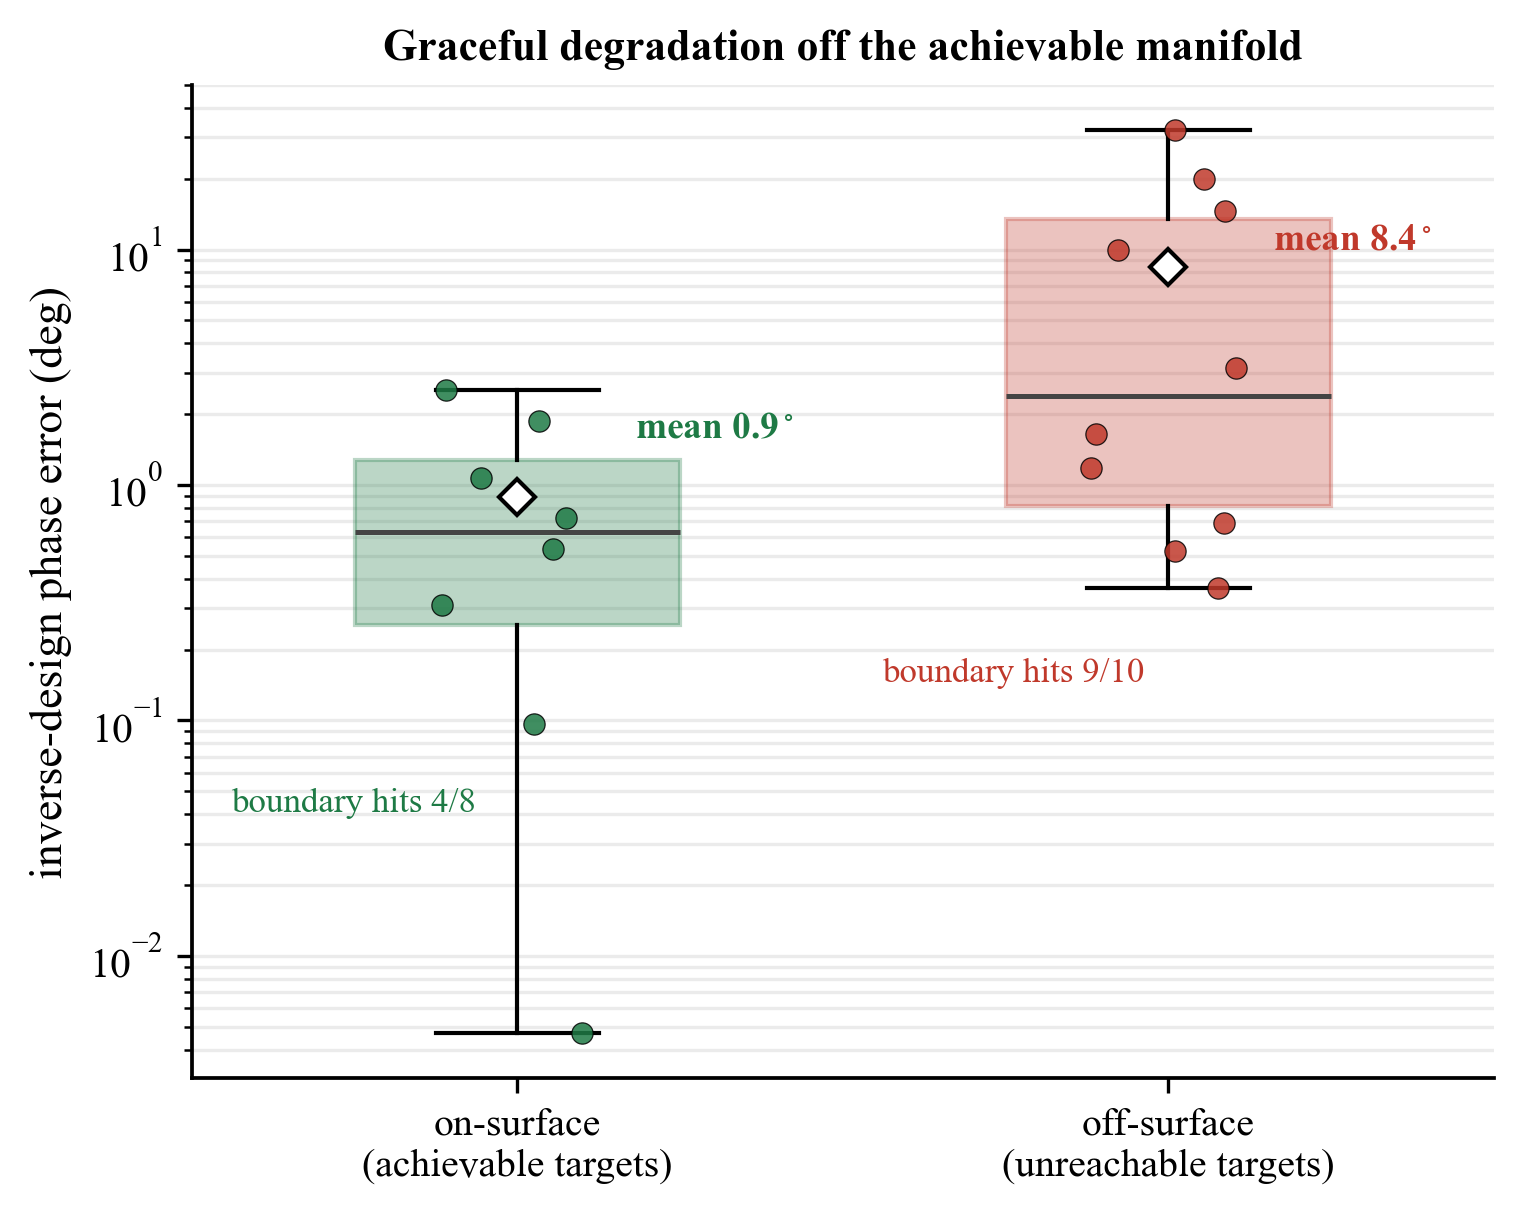
\includegraphics[width=0.6\linewidth]{fig_p3_ood.png}
\caption{Inverse-design robustness. On-surface (achievable) targets are hit to $\sim$\SI{0.9}{\degree};
deliberately off-surface / over-specified targets degrade gracefully to $\sim$\SI{8.4}{\degree}, with the
solution pinned to the design-box boundary in $9/10$ cases (vs $4/8$ on-surface)---predictable failure,
not a confident wrong answer.}
\label{fig:ood}
\end{figure}

\begin{table}[!ht]\centering\small
\caption{Two-parameter inverse design. Eight target reflections (phase and magnitude drawn from the
achievable surface), the surrogate-solved geometry, and the openEMS-verified achieved values.}
\label{tab:inverse}
\begin{tabular}{cccccccc}
\toprule
target $\angle\Gamma$ & target $|\Gamma|$ & solved $L_x$ & solved $L_y$ & achieved $\angle\Gamma$ &
phase err & $|\Gamma|$ err \\
(deg) & & (mm) & (mm) & (deg) & (deg) & \\
\midrule
$-152.1$ & 0.97 & 4.26 & 4.74 & $-150.3$ & 1.87 & 0.01 \\
$-123.5$ & 0.94 & 5.34 & 2.44 & $-122.5$ & 1.07 & 0.00 \\
$-94.9$  & 0.85 & 6.00 & 2.13 & $-92.4$  & 2.53 & 0.03 \\
$-66.3$  & 0.81 & 5.02 & 2.01 & $-66.0$  & 0.31 & 0.00 \\
$-37.7$  & 0.72 & 3.63 & 2.01 & $-37.0$  & 0.72 & 0.01 \\
$-9.2$   & 0.69 & 3.00 & 2.00 & $-9.2$   & 0.00 & 0.00 \\
$+19.4$  & 0.68 & 2.51 & 2.00 & $+19.5$  & 0.10 & 0.00 \\
$+48.0$  & 0.73 & 2.15 & 2.00 & $+47.5$  & 0.53 & 0.01 \\
\midrule
\multicolumn{5}{r}{mean} & \textbf{0.89} & \textbf{0.01} \\
\bottomrule
\end{tabular}
\end{table}

\section{Ablation: is the physics residual needed?}\label{sec:abl}
We finally test whether a Maxwell-residual term helps, on the square-patch task where the same resonance
appears (Fig.~\ref{fig:ablation}). A data-free PINN (Maxwell residual only) cannot represent the
resonance: its reflection phase stays essentially flat, with a resonance-region error of
\SI{91.8}{\degree}. Adding the same sparse anchors as a physics-informed \emph{hybrid} does not rescue
it---and at matched anchors it is \emph{worse} than pure data (\SI{35}{\degree} for the best hybrid
versus \SI{1.2}{\degree} for the identical anchors used as pure resonance-aware data). We verified this
across the hybrid's design choices (data-loss weight, physics-weight annealing, additional cavity
collocation): the only adjustments that improved the hybrid were those that \emph{suppressed} the
physics term, i.e.\ that moved it back toward pure regression. The result is not an artefact of a naive
fixed loss weight. We also tested an \emph{advanced} hybrid with NTK/gradient-norm adaptive weighting,
which rescales the data and physics terms so neither dominates by parameter-gradient
magnitude~\cite{wanggrad2021}: on the two-parameter family at the matched $12$ anchors it reaches
\SI{68.9}{\degree} resonance error---still $\sim\!26\times$ worse than the same anchors used as pure data
(\SI{2.66}{\degree}). Principled gradient balancing therefore does not rescue the hybrid. We do not test a
scattered-field reformulation or causal/curriculum training, and we restrict the claim to total-field
formulations on this low-dimensional, data-cheap task.

The mechanism is the known PINN failure
mode~\cite{krishnapriyan2021}: for an under-resolved, high-$Q$ field the
Maxwell-residual's low-data optimum is the smooth, non-resonant field, so the residual acts as an
\emph{anti-regulariser}, pulling the fit off the correct resonant interpolation that the data alone
would reach---a soft-constraint Pareto tension in which the physics and data optima do not coincide.
For this resonant unit-cell response, then, the effective lever is data placement, not the physics
residual---a concrete electromagnetic instance of when physics-informed regularisation does not help,
complementing the general failure-mode analyses with a device-level, quantified case.

\paragraph{The result holds in a higher-dimensional, data-scarcer regime.} A fair objection is that the
ablation above is on the easy one-parameter (square-patch $L$) family, where data is cheapest---precisely
the regime least favourable to a data-free PINN. We therefore repeat it on the full \emph{two-parameter}
$(L_x,L_y)$ geometry family (rectangular patch, $h$ fixed), with only $12$ resonance-aware anchors over the
$99$-point surface---higher dimension and sparser data, where a physics prior should help most. The
conclusion is unchanged and in fact sharper: the data-free PINN still fails (resonance-region error
\SI{99.4}{\degree}, phase essentially flat), the physics+data hybrid at the matched $12$ anchors is far
worse than pure data (\SI{82.2}{\degree} vs \SI{2.66}{\degree}, a $\sim\!31\times$ gap), and pure
resonance-aware regression on the same anchors is best. The Maxwell residual remains an anti-regulariser as
the geometry dimension grows; well-placed data is the lever in both the one- and two-parameter regimes.
This does not claim universality across all formulations, but it removes the ``only true in the easy 1-D
case'' caveat.

\begin{figure}[!htbp]\centering
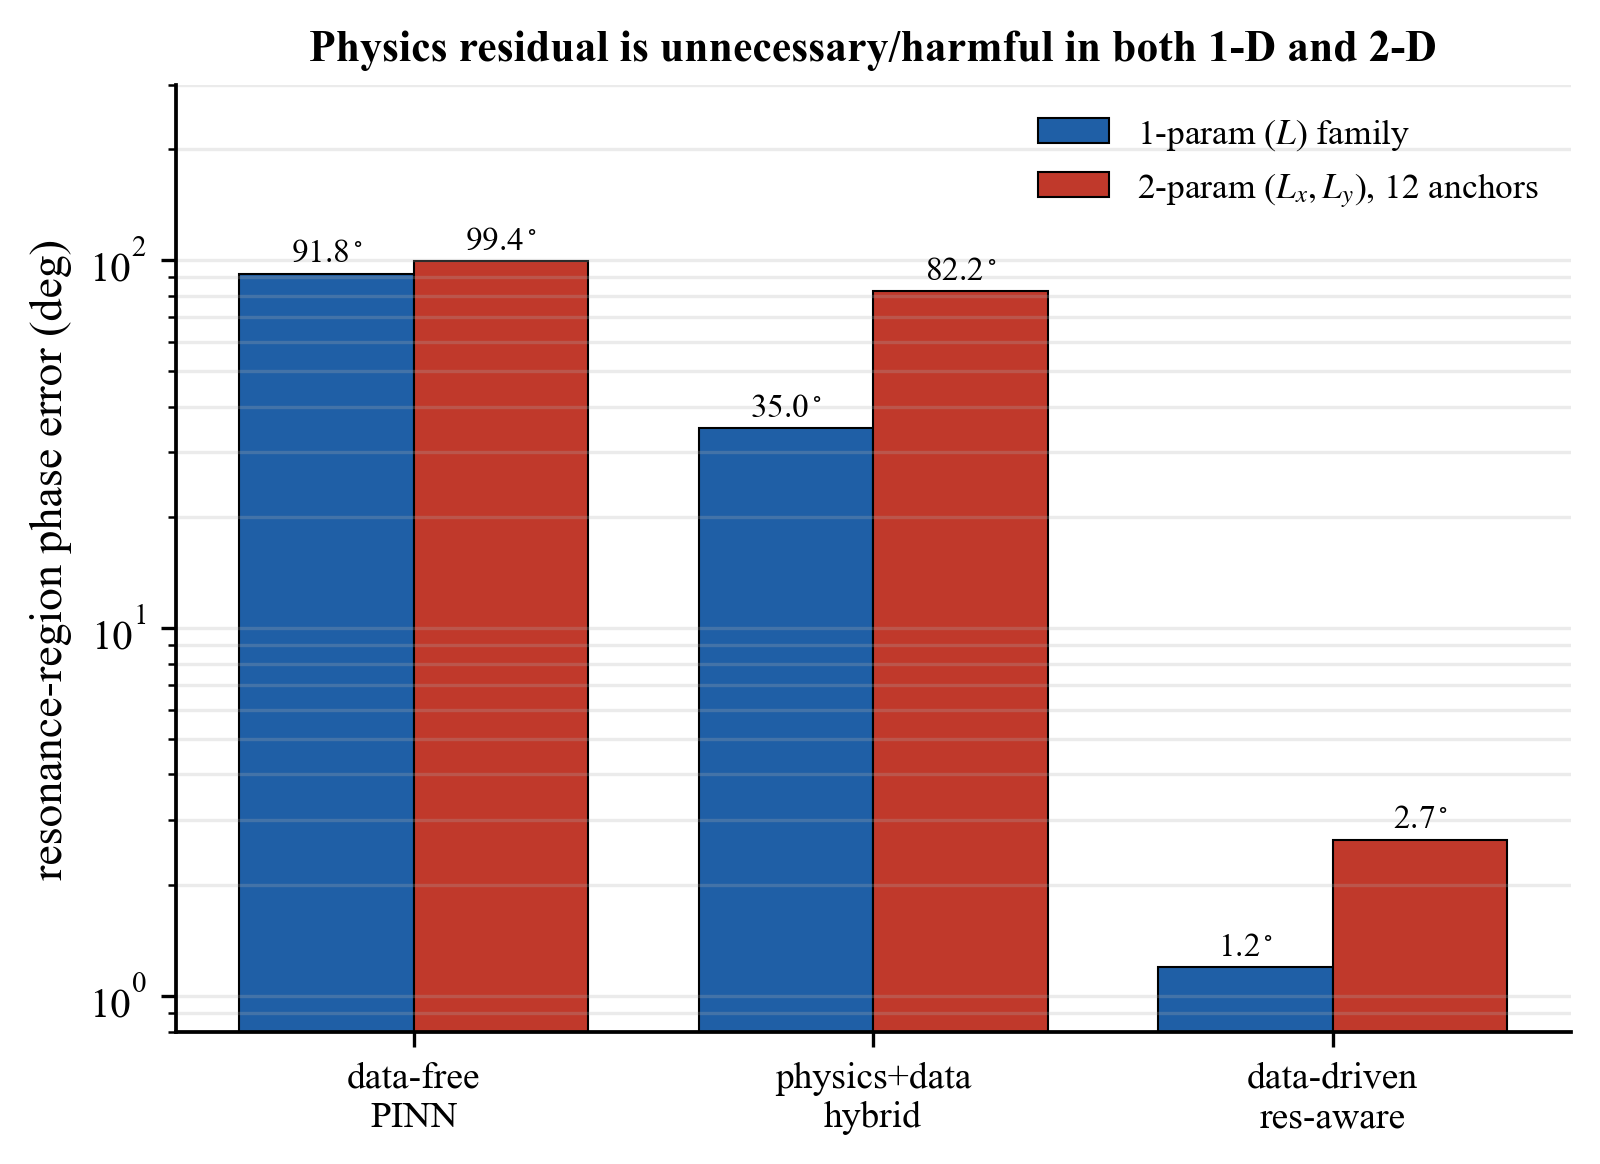
\includegraphics[width=0.62\linewidth]{fig_p3_ablation.png}
\caption{Ablation (resonance-region phase error, log scale) on \emph{both} the one-parameter ($L$)
square-patch family and the higher-dimensional, data-scarcer two-parameter $(L_x,L_y)$ family (12
anchors). In both, a data-free PINN is flat, a physics+data hybrid is worse than pure data at matched
anchors, and resonance-aware data is best---the physics residual is unnecessary and counterproductive, and
the gap \emph{widens} in 2-D ($\sim\!31\times$). An advanced NTK/gradient-norm-balanced hybrid (not plotted)
remains $\sim\!26\times$ worse than pure data, so the result is not a naive-loss-weight artefact.}
\label{fig:ablation}
\end{figure}

\section{Aperture-level demonstration: full-wave anomalous reflection}\label{sec:steer}
What this section delivers is the \emph{pipeline closure}, not the grating: we test whether the
surrogate$\to$geometry$\to$full-wave loop closes and whether the deflection \emph{angle} is controllable by
design. Aperture \emph{efficiency} is out of scope here (and reported honestly as a limitation),
because a single-resonance cell cannot deliver it; the evidence task is angle control through the
differentiable model, end to end. To that end we close the loop with a full-wave \emph{anomalous-reflection}
demonstration (a coded metagrating, not a fed reflectarray). A linear reflection-phase ramp of
super-period $\Lambda=Mp$ ($p$ the cell pitch) deflects a normally-incident plane wave into the anomalous
order $\theta=\arcsin(\lambda_0/\Lambda)$ by the generalized Snell law~\cite{yu2011,sun2012}; choosing the
super-period $M$ at \emph{design time} selects the deflection angle (this is geometric re-coding, not
runtime/reconfigurable steering). We synthesise the ramp by inverting the surrogate's size$\to$phase
map---the same differentiable model of the preceding sections---to pick each cell size, and we close it in
openEMS on a multi-super-period strip with periodic walls and a normally-incident plane wave, isolating
the reflected field by a per-column two-plane decomposition and reading the diffraction orders by a
spatial Fourier transform.

The full-wave anomalous order is aimed almost exactly where predicted
(Table~\ref{tab:steer}, Fig.~\ref{fig:steer}): as $M$ runs $8\!\to\!3$ its angle scans
$11.3^\circ\!\to\!31.7^\circ$, within $\approx\!\SI{0.3}{\degree}$ of generalized Snell at every point.
This angle control is what a high-$Q$ Fabry--P\'erot cavity cannot provide. We report efficiency without
embellishment, and note it does \emph{not} make this a usable aperture. The anomalous order carries only
$\approx\!29$--$39\%$ of the power, and at small $M$ ($M\!=\!3,4,5$) the specular ($m{=}0$) order actually
carries \emph{more} ($52/42/44\%$); the anomalous lobe is correctly aimed but is not dominant there. Two
causes compound: a single patch realises only $211^\circ$ of reflection phase along a 1-D size cut
($259^\circ$ at $h{=}\SI{1.5}{mm}$; the full 2-D $(L_x,L_y)$ surface spans $222^\circ$), short of the
$360^\circ$ a blaze needs; and---as the metasurface-efficiency
literature establishes---full $360^\circ$ phase coverage is \emph{necessary but not sufficient}, because
local phase-gradient (generalized-Snell) designs suffer impedance-mismatch loss that grows with
deflection angle, so reaching high efficiency requires non-local/strongly-coupled
elements~\cite{diazrubio2017}; the lossy FR4 ($\tan\delta=0.02$, $|\Gamma|$ down to $0.68$) imposes a
further ceiling. The result is therefore a \emph{proof-of-pipeline}: the surrogate-synthesised code aims
the full-wave anomalous order to $\SI{0.3}{\degree}$, while delivering a usable-efficiency aperture is a
separate (non-local element) design problem.

The per-super-period angle-and-efficiency breakdown is tabulated in Appendix~\ref{app:steer}
(Table~\ref{tab:steer}).

\begin{figure}[!htbp]\centering
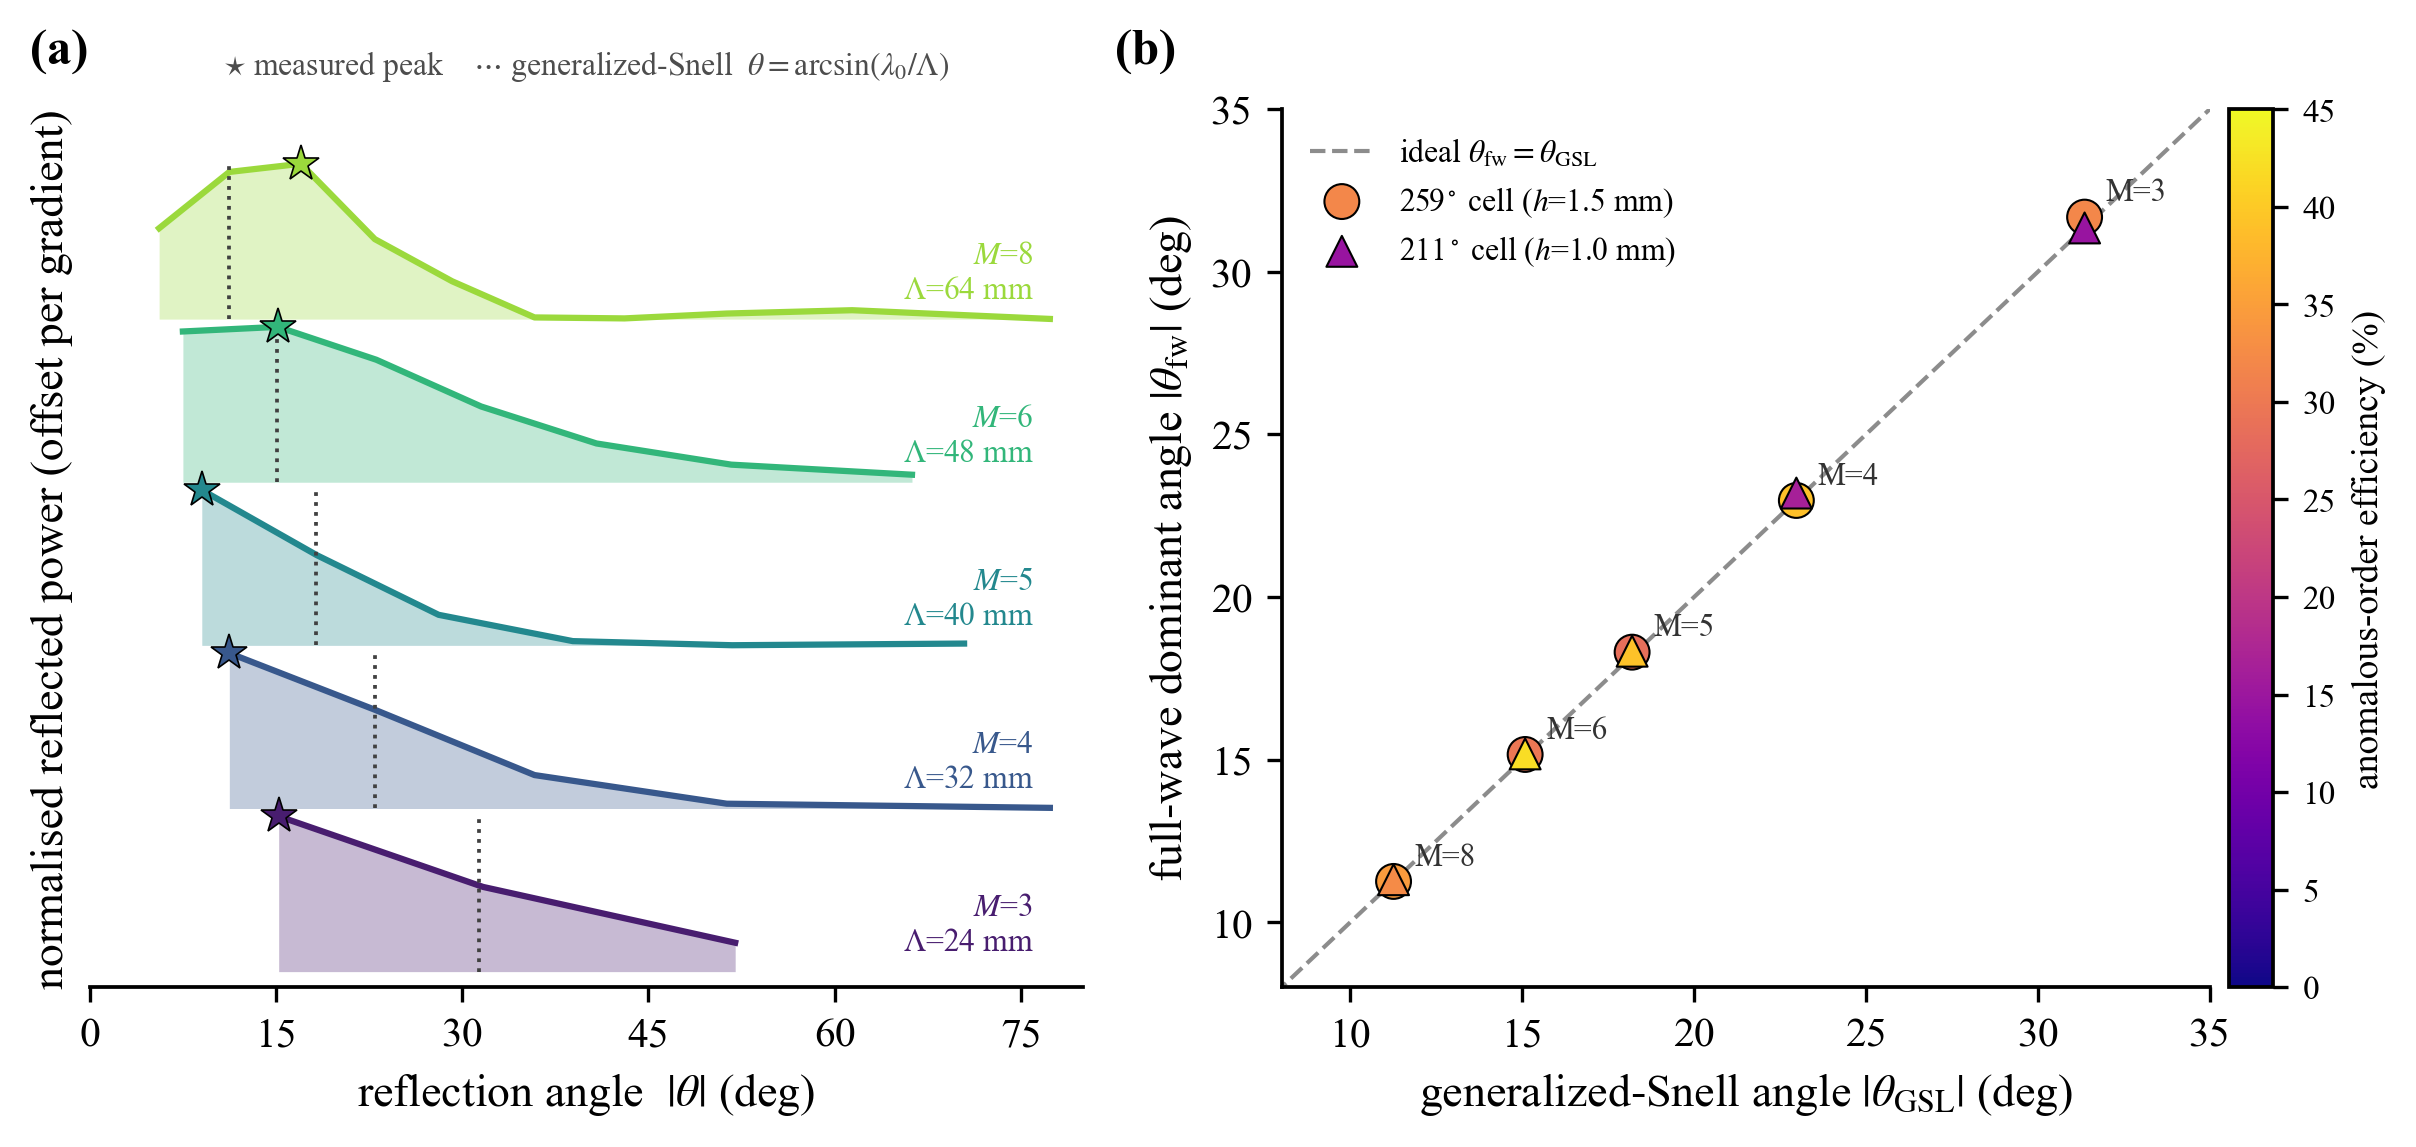
\includegraphics[width=0.98\linewidth]{fig_meta_steer.png}
\caption{Full-wave anomalous reflection. Reflected power versus angle for surrogate-synthesised phase-gradient
codings of decreasing super-period; the anomalous lobe scans $\approx\!11^\circ\!\to\!32^\circ$ and its
peak tracks the generalized-Snell angle (markers). The steer angle is re-codable by the coding period.}
\label{fig:steer}
\end{figure}

\section{Discussion}\label{sec:disc}
We draw out three messages. First, for sub-wavelength resonant cells the dominant cost---full-wave
characterisation---is minimised not by a cleverer learner but by \emph{where} the few samples are
placed: resonance-aware active sampling cuts the resonance-region error by an order of magnitude at
fixed budget and steepens the error-versus-budget law from $N^{-0.8}$ to $N^{-2.1}$. This specialises
general error-driven active learning for photonic surrogates~\cite{pestourie2020} to a simple,
resonance-targeted curvature/uncertainty criterion---demonstrated here on the microwave reflectarray cell
and, changing only the oracle, shown to transfer to non-electromagnetic resonance-dominated responses
(a driven-oscillator/RLC line shape and a Fano resonance, Section~\ref{sec:outdomain}), evidence that the
criterion is not specific to electromagnetics---and
pairs it with a \emph{differentiable} model so the same surrogate serves inverse design. Second, the sampling strategy
and the learner are coupled: the active anchors that help the differentiable network actively hurt a
global-kernel support-vector model, so ``use active learning'' is incomplete advice without ``with a
learner that tolerates clustered data.'' Third, the physics residual---attractive because it needs no
data---is the wrong tool for this response: it fails alone and degrades the data fit when added,
consistent with PINN stiffness and spectral-bias
analyses~\cite{wang2021ntk,tancik2020}. We are careful not to overgeneralise:
this is established for a \emph{low-dimensional, total-field} formulation of one resonant cell, a regime
where data is cheap and pure regression is already strong; a scattered-field reformulation (see the
outlook below) may avoid the anti-regularisation, and the PINN value proposition (no data, higher dimension) is
not what this testbed probes. The conditional lesson---for this class of low-dimensional resonant
responses, a total-field Maxwell residual does not help and can hurt---is what we claim.

\paragraph{Scope and threats to validity.} We state the boundaries of every claim explicitly. (1)~The
study is \emph{simulation-only} with a full-wave (not measured) baseline; no measured hardware is reported.
(2)~A \emph{single} full-wave solver (openEMS) is the reference throughout, so solver-specific bias is not
ruled out, though it is independently spot-checked (a square-patch cross-check agreeing to $\sim\!4^\circ$
and the fine finite-difference gradient audit of Section~\ref{sec:grad}). (3)~The physics-residual ablation
uses a \emph{total-field} formulation only; a scattered-field reformulation is untested and may behave
differently. (4)~The off-electromagnetic transfer (Section~\ref{sec:outdomain}) uses \emph{analytic}
oracles, so it demonstrates that the acquisition \emph{criterion} transfers, \emph{not} that it saves cost
on an expensive non-EM solver; the cost-saving claims are confined to the simulated reflectarray testbed.
(5)~The aperture-level result is a \emph{proof-of-pipeline} (angle correct to $\approx\!\SI{0.3}{\degree}$;
anomalous-order efficiency $29$--$39\%$), not a usable-aperture claim. Within these bounds, the quantified
claims carry their uncertainty: every reported scaling exponent is given with a bootstrap 95\% confidence
interval over seeds (Tables~\ref{tab:scaling},~\ref{tab:3d}), and the data-efficiency dominance is stated as
holding outside the per-budget $\pm$std bands rather than as a bare point estimate.

For a \emph{sampling-and-surrogate methodology} the full-wave reference is the correct and standard one---the
method's job is to reproduce the solver from few calls, exactly as in prior active-learning surrogate work
that validates against the solver~\cite{pestourie2020}---and hardware measurement is the natural next
milestone rather than a gap in the present claim. Beyond this, the cell is parameterised by two
dimensions, and the magnitude near resonance is intrinsically less controllable than the phase because
$|\Gamma|$ physically dips there. Natural extensions are higher-dimensional cells (adding, e.g., a slot
or a dielectric-thickness degree of freedom, where the differentiable gradient and curvature-driven
sampling should matter more), a full coded-aperture closure that chains the cell surrogate into an
array-level inverse design, and a reformulated physics term acting on the scattered (rather than total)
field, which may avoid the anti-regularisation identified here.

\section{Conclusion}
A lightweight, data-driven, \emph{differentiable} surrogate trained on $\mathcal{O}(10)$ full-wave
anchors placed by resonance-aware active sampling models the complete two-parameter reflection-phase
surface of a 24-GHz reflectarray cell, beats standard surrogates at equal sample budgets under active
sampling, supplies full-wave-consistent geometry gradients, and drives a two-parameter inverse-design
loop to \SI{0.9}{\degree} accuracy. A controlled ablation shows the Maxwell-residual term is unnecessary
and, for this resonant response, counterproductive---the lever is data placement. The outcome is a
transferable methodology---resonance-aware active learning plus a differentiable surrogate, with a
quantified data-efficiency law and a device-level negative result on physics-informed regularisation---for
expensive-to-sample, resonance-dominated parametric responses, here instantiated and validated end to end
as a data-efficient, differentiable unit-cell design tool, with each method choice justified by direct
comparison. We demonstrate it on one reflectarray cell class in simulation and claim no universality
beyond that.

\section*{CRediT authorship contribution statement}
\textbf{Long Zhang}: Conceptualization, Methodology, Software, Investigation, Writing -- original draft,
Supervision, Funding acquisition.
\textbf{Xuan Shi}: Software, Formal analysis, Validation.
\textbf{Liang Ma}: Data curation, Visualization.
\textbf{Shengjun Wu}: Methodology, Resources.
\textbf{Kai You}: Validation, Resources.
\textbf{Zijuan Wu}: Validation, Writing -- review \& editing.

\section*{Declaration of competing interest}
The authors declare no competing interest.

\section*{Funding}
This work was supported by the Doctoral Scientific Research Foundation of Hubei University of Automotive
Technology (Grant No.\ BK2023536), the Open Fund of the Hubei Key Laboratory of Automotive Power Train and
Electronic Control (Grant No.\ ZDK1202004), the Hubei Provincial Collaborative Innovation Center for
Automotive Components Technology (Grant No.\ 2015XTZX0421), and the Open Fund of the Zhejiang Provincial Key
Laboratory of Intelligent Construction and Maintenance for Deep-Sea Infrastructure (Grant No.\ SJ202512).

\section*{Ethics and consent}
Not applicable.

\section*{Data availability}
The openEMS full-wave reference (the 99-point 2-D and 324-point 3-D $(L_x,L_y,h)$ grids and the metagrating
closures), the trained surrogate, the active-sampling/baseline/gradient/inverse scripts, and the
figure/table generators are openly available at
\url{https://github.com/zlera20230100/reflectarray-surrogate} and archived on Zenodo
(DOI: \href{https://doi.org/10.5281/zenodo.20809888}{10.5281/zenodo.20809888}).

\section*{Declaration of generative AI and AI-assisted technologies in the writing process}
During the preparation of this work the authors used a large-language-model-based assistant \emph{solely to
improve the language and readability} of the manuscript. After using this tool, the authors reviewed and
edited the content as needed and take full responsibility for the content of the publication. No
generative-AI tool was used to generate scientific content, data, figures, or analysis, and no AI tool is
listed as an author.

\appendix
\section{Full-wave reference: openEMS configuration}\label{app:openems}
The reference surfaces are computed with openEMS (FDTD) in a waveguide-simulator unit cell. Excitation: a
Gaussian pulse centred at $f_0=\SI{24}{GHz}$ with $\SI{12}{GHz}$ half-bandwidth, applied as a
$y$-polarised plane-wave field source on a plane above the cell; fields are read in the frequency domain at
$f_0$. Boundaries realise normal incidence with $\mathbf{E}\parallel y$: magnetic walls (PMC) $\perp x$,
electric walls (PEC) $\perp y$, a PEC ground plane at $z=0$, and an $8$-cell PML above the cell. The run
terminates at an energy-decay criterion of $10^{-5}$ (cap $6\times10^{4}$ time steps). The mesh pins explicit
lines to the patch edges ($\pm L_x/2,\pm L_y/2$) and to the two readout planes, is smoothed to a maximum
adjacent-cell ratio of $0.35$, and near-coincident lines ($<\!\SI{e-3}{mm}$) are de-duplicated to avoid
sliver cells and tiny time steps. Materials: grounded FR4 ($\varepsilon_r=4.4$, $\tan\delta=0.02$,
conductivity $\kappa=2\pi f_0\varepsilon_0\varepsilon_r\tan\delta$), thickness $h=\SI{1}{mm}$, period
$p=\SI{8}{mm}$; PEC patch and ground. The reflection coefficient is extracted by sampling the mean $E_y$ on
two air-region planes $z_1=\SI{5}{mm}$, $z_2=\SI{6.5}{mm}$ (each $>\!0.3\lambda_0$ above the patch) and
solving the traveling-wave system of Eq.~\eqref{eq:twoplane} for $\Gamma=A/B$, referenced to the ground
plane. The 2-D sweep is $L_y\in\mathrm{linspace}(2,6,11)$, $L_x\in\mathrm{linspace}(2,6,9)=99$ simulations;
the 3-D study adds $h$ on a $9\times9\times4=324$ grid; the cross-dipole and dual-resonance cells use the
same simulator with the metal redefined. Exact scripts are in the released repository.

\section{Total-field PINN ablation: residual and boundary treatment}\label{app:pinn}
The ablation (Section~\ref{sec:abl}) models a geometry-conditioned \emph{scalar total field}
$E_y(x,y,z;L)$ with an MLP and minimises the residual of the scalar Helmholtz equation---the $y$-component
of the curl--curl equation under the waveguide-simulator polarisation---in the air/dielectric region,
\begin{equation}
\mathcal{R}(x,y,z;L)=\nabla^2 E_y + k_0^2\,\varepsilon_r(x,y,z;L)\,E_y ,
\label{eq:pinnres}
\end{equation}
where the cell geometry enters through a (smoothed) permittivity indicator $\varepsilon_r(\cdot;L)$ that
encodes the patch/dielectric region as a function of the size parameters $L$. Boundary and excitation terms
are imposed as soft penalties: $E_y=0$ on the PEC ground plane and patch metal, the waveguide-simulator wall
conditions (PMC $\perp x$, PEC $\perp y$), and an incident-field condition at the top plane reproducing the
plane-wave drive; the reflection $\Gamma$ is read from the network by the \emph{same} two-plane
decomposition (Eq.~\eqref{eq:twoplane}) used for the full-wave reference, so the data loss
(Eq.~\eqref{eq:data}) and the physics residual share one observable. The data-free PINN minimises
Eq.~\eqref{eq:pinnres} plus boundary/excitation terms only; the hybrid adds Eq.~\eqref{eq:data} on the
anchor set; the advanced hybrid additionally rescales the data and physics terms by NTK/gradient-norm
adaptive weights~\cite{wanggrad2021}. Collocation points are a structured grid over the air$+$dielectric
region, de-weighted near the source plane. Loss weights, physics-weight annealing, and collocation counts
were swept (Section~\ref{sec:abl}); the only adjustments that improved the hybrid were those that suppressed
the physics term. All hyperparameters are in the released code.

\section{Anomalous-reflection closure: per-super-period breakdown}\label{app:steer}
Table~\ref{tab:steer} gives the full angle-and-efficiency data for the anomalous-reflection closure of
Section~\ref{sec:steer}. The anomalous-order angle tracks generalized Snell's law to
$\approx\!\SI{0.3}{\degree}$ at every super-period; efficiency is reported honestly: at small super-period
($M{=}3,4,5$) the specular ($m{=}0$) order carries \emph{more} power than the aimed anomalous order---the
angle is correct but not dominant, consistent with the single-resonance phase coverage and the
non-local-element requirement discussed in Section~\ref{sec:steer}.

\begin{table}[!ht]\centering\small
\caption{Full-wave anomalous reflection by a surrogate-synthesised phase-gradient metagrating
($\SI{259}{\degree}$ cell, $h=\SI{1.5}{mm}$); angles as magnitudes, the order sign alternating with $M$.}
\label{tab:steer}
\begin{tabular}{cccccc}
\toprule
$M$ & $\Lambda$ (mm) & GSL angle (deg) & full-wave angle (deg) & anomalous eff. & specular ($m{=}0$) \\
\midrule
8 & 64 & 11.26 & 11.25 & 35\% & 10\% \\
6 & 48 & 15.08 & 15.16 & 30\% & 25\% \\
5 & 40 & 18.20 & 18.30 & 29\% & 44\% \\
4 & 32 & 22.98 & 22.97 & 39\% & 42\% \\
3 & 24 & 31.36 & 31.69 & 32\% & 52\% \\
\bottomrule
\end{tabular}
\end{table}

\begin{thebibliography}{99}
\small
\bibitem{trentini1956} G.~von Trentini, ``Partially reflecting sheet arrays,'' \emph{IRE Trans. Antennas Propag.} 4(4):666--671, 1956.
\bibitem{cui2014} T.J. Cui, M.Q. Qi, X. Wan, J. Zhao, Q. Cheng, ``Coding metamaterials, digital metamaterials and programmable metamaterials,'' \emph{Light Sci. Appl.} 3:e218, 2014.
\bibitem{reflectarray2022} A.V. Diebold, D. Pande, C. Gregg, D.R. Smith, ``Reflectarray design using a discrete dipole framework,'' arXiv:2206.00095, 2022.
\bibitem{li2021codingreflector} W. Li, T. Qiu, J. Wang, L. Zheng, Y. Jing, Y. Jia, H. Wang, Y. Han, S. Qu, ``Programmable coding metasurface reflector for reconfigurable multibeam antenna application,'' \emph{IEEE Trans. Antennas Propag.} 69(1):296--301, 2021.
\bibitem{abdelrahman2015transmitarray} A.H. Abdelrahman, P. Nayeri, A.Z. Elsherbeni, F. Yang, ``Bandwidth improvement methods of transmitarray antennas,'' \emph{IEEE Trans. Antennas Propag.} 63(7):2946--2954, 2015.
\bibitem{epstein2014huygens} A. Epstein, G.V. Eleftheriades, ``Passive lossless Huygens metasurfaces for conversion of arbitrary source field to directive radiation,'' \emph{IEEE Trans. Antennas Propag.} 62(11):5680--5695, 2014.
\bibitem{ludeeponet2021} L. Lu, P. Jin, G. Pang, Z. Zhang, G.E. Karniadakis, ``Learning nonlinear operators via DeepONet,'' \emph{Nat. Mach. Intell.} 3:218--229, 2021.
\bibitem{li2021fno} Z. Li, N. Kovachki, K. Azizzadenesheli, B. Liu, K. Bhattacharya, A. Stuart, A. Anandkumar, ``Fourier neural operator for parametric partial differential equations,'' \emph{ICLR}, 2021 (arXiv:2010.08895).
\bibitem{augenstein2023} Y. Augenstein, T. Rep\"an, C. Rockstuhl, ``Neural operator-based surrogate solver for free-form electromagnetic inverse design,'' \emph{ACS Photonics} 10(5):1547--1557, 2023.
\bibitem{jiang2021} J. Jiang, M. Chen, J.A. Fan, ``Deep neural networks for the evaluation and design of photonic devices,'' \emph{Nat. Rev. Mater.} 6:679--700, 2021.
\bibitem{koziel2024surrogate} S. Koziel, A. Pietrenko-Dabrowska, L. Leifsson, ``Antenna optimization using machine learning with reduced-dimensionality surrogates,'' \emph{Sci. Rep.} 14:21567, 2024.
\bibitem{sarker2023mlreview} N. Sarker, P. Podder, M.R.H. Mondal, S.S. Shafin, J. Kamruzzaman, ``Applications of machine learning and deep learning in antenna design, optimization, and selection: a review,'' \emph{IEEE Access} 11:103890--103915, 2023.
\bibitem{pestourie2020} R. Pestourie, Y. Mroueh, T.V. Nguyen, P. Das, S.G. Johnson, ``Active learning of deep surrogates for PDEs: application to metasurface design,'' \emph{npj Comput. Mater.} 6:164, 2020 (arXiv:2008.12649).
\bibitem{settles2012} B. Settles, \emph{Active Learning}, Synthesis Lectures on Artificial Intelligence and Machine Learning, Morgan \& Claypool, 2012.
\bibitem{lookman2019} T. Lookman, P.V. Balachandran, D. Xue, R. Yuan, ``Active learning in materials science with emphasis on adaptive sampling using uncertainties for targeted design,'' \emph{npj Comput. Mater.} 5:21, 2019.
\bibitem{crombecq2011} K. Crombecq, D. Gorissen, D. Deschrijver, T. Dhaene, ``A novel hybrid sequential design strategy for global surrogate modeling of computer experiments,'' \emph{SIAM J. Sci. Comput.} 33(4):1948--1974, 2011.
\bibitem{gramacy2020} R.B. Gramacy, \emph{Surrogates: Gaussian Process Modeling, Design, and Optimization for the Applied Sciences}, Chapman \& Hall/CRC, 2020.
\bibitem{sener2018} O. Sener, S. Savarese, ``Active learning for convolutional neural networks: a core-set approach,'' in \emph{Int. Conf. on Learning Representations (ICLR)}, 2018.
\bibitem{liu2018} D. Liu, Y. Tan, E. Khoram, Z. Yu, ``Training deep neural networks for the inverse design of nanophotonic structures,'' \emph{ACS Photonics} 5(4):1365--1369, 2018.
\bibitem{molesky2018} S. Molesky, Z. Lin, A.Y. Piggott, W. Jin, J. Vu\v{c}kovi\'c, A.W. Rodriguez, ``Inverse design in nanophotonics,'' \emph{Nat. Photonics} 12:659--670, 2018.
\bibitem{raissi2019} M. Raissi, P. Perdikaris, G.E. Karniadakis, ``Physics-informed neural networks,'' \emph{J. Comput. Phys.} 378:686--707, 2019.
\bibitem{karniadakis2021} G.E. Karniadakis, I.G. Kevrekidis, L. Lu, P. Perdikaris, S. Wang, L. Yang, ``Physics-informed machine learning,'' \emph{Nat. Rev. Phys.} 3:422--440, 2021.
\bibitem{beltran2022} A. Beltr\'an-Pulido, I. Bilionis, D. Aliprantis, ``Physics-informed neural networks for solving parametric magnetostatic problems,'' \emph{IEEE Trans. Energy Convers.} 37(4):2678--2689, 2022.
\bibitem{nohra2024pinnem} M. Nohra, S. Dufour, ``Physics-informed neural networks for the numerical modeling of steady-state and transient electromagnetic problems with discontinuous media,'' arXiv:2406.04380, 2024.
\bibitem{krishnapriyan2021} A.S. Krishnapriyan, A. Gholami, S. Zhe, R.M. Kirby, M.W. Mahoney, ``Characterizing possible failure modes in physics-informed neural networks,'' \emph{NeurIPS}, 2021.
\bibitem{wang2021ntk} S. Wang, X. Yu, P. Perdikaris, ``When and why PINNs fail to train: a neural tangent kernel perspective,'' \emph{J. Comput. Phys.} 449:110768, 2022.
\bibitem{wanggrad2021} S. Wang, Y. Teng, P. Perdikaris, ``Understanding and mitigating gradient flow pathologies in physics-informed neural networks,'' \emph{SIAM J. Sci. Comput.} 43(5):A3055--A3081, 2021.
\bibitem{tancik2020} M. Tancik et al., ``Fourier features let networks learn high frequency functions in low dimensional domains,'' \emph{NeurIPS} 33:7537--7547, 2020.
\bibitem{yu2011} N. Yu, P. Genevet, M.A. Kats, F. Aieta, J.-P. Tetienne, F. Capasso, Z. Gaburro, ``Light propagation with phase discontinuities: generalized laws of reflection and refraction,'' \emph{Science} 334(6054):333--337, 2011.
\bibitem{sun2012} S. Sun, Q. He, S. Xiao, Q. Xu, X. Li, L. Zhou, ``Gradient-index meta-surfaces as a bridge linking propagating waves and surface waves,'' \emph{Nat. Mater.} 11(5):426--431, 2012.
\bibitem{diazrubio2017} A. D\'iaz-Rubio, V.S. Asadchy, A. Elsakka, S.A. Tretyakov, ``From the generalized reflection law to the realization of perfect anomalous reflectors,'' \emph{Sci. Adv.} 3(8):e1602714, 2017.
\bibitem{pozar1997} D.M. Pozar, S.D. Targonski, H.D. Syrigos, ``Design of millimeter wave microstrip reflectarrays,'' \emph{IEEE Trans. Antennas Propag.} 45(2):287--296, 1997.
\bibitem{robustillo2012} P. Robustillo, J. Zapata, J.A. Encinar, J. Rubio, ``ANN characterization of multi-layer reflectarray elements for contoured-beam space antennas in the Ku-band,'' \emph{IEEE Trans. Antennas Propag.} 60(7):3205--3214, 2012.
\bibitem{prado2018} D.R. Prado, J.A. L\'opez-Fern\'andez, G. Barquero, M. Arrebola, F. Las-Heras, ``Fast and accurate modeling of dual-polarized reflectarray unit cells using support vector machines,'' \emph{IEEE Trans. Antennas Propag.} 66(3):1258--1270, 2018.
\end{thebibliography}

\end{document}
